\documentclass[a4paper,12pt]{report}
\usepackage[utf8]{inputenc}
\usepackage[sfdefault]{roboto}

\usepackage{titling}
\usepackage{graphicx}
\usepackage{wrapfig}
\usepackage{subcaption}
\usepackage{float}
\usepackage{fontawesome}
\usepackage{setspace}
\usepackage[export]{adjustbox}
\usepackage[margin=20mm]{geometry}
\usepackage{soul}

\usepackage{xcolor}
\definecolor{turbo_purple}{RGB}{112,105,160}
\definecolor{sponsor_bronze}{RGB}{205,127,50}
\definecolor{sponsor_silver}{RGB}{170,169,173}
\definecolor{sponsor_gold}{RGB}{212,175,55}

\usepackage{titlesec}
\titleformat{\section}[block]{\normalfont\huge\bfseries\centering}{}{1em}{}
\titleformat{\subsection}[display]{\normalfont\Large\bfseries\color{turbo_purple}}{}{1em}{}
\titleformat{\subsubsection}[display]{\normalfont\large\bfseries}{}{}{\vspace{-1.2em}}[\vspace{-0.9em}]

\usepackage{fancyhdr}
\pagestyle{fancy}
\usepackage{tikz}
\usetikzlibrary{calc}
\usepackage{tikzpagenodes}
\fancyfoot{}
\renewcommand{\headrulewidth}{0pt}
\setlength{\headheight}{25pt}
\rhead{\begin{tikzpicture}[remember picture,overlay]
\draw  let \p1=($(current page.north)-(current page header area.south)$),
      \n1={veclen(\x1,\y1)} in
node [inner sep=0,outer sep=0,below left] 
      at (current page.north east){
\includegraphics[height=\n1]{../assets/Sponsorship Header - Solid.png}};
\end{tikzpicture}}
\lfoot{\begin{tikzpicture}[remember picture,overlay]
\draw  let \p1=($(current page footer area.north)-(current page.south)$),
      \n1={veclen(\x1,\y1)} in
node [inner sep=0,outer sep=0,above right] 
      at (current page.south west){
\includegraphics[height=\n1]{../assets/Sponsorship Footer - Solid.png}};
\end{tikzpicture}}
\cfoot{\sffamily\selectfont\thepage}

\usepackage[hidelinks]{hyperref}
\hypersetup{colorlinks=false}

\begin{document}

\begin{titlepage}
    \newgeometry{right=0mm,left=0mm,top=20mm,bottom=0mm}
    \begin{center}
        \vspace*{15mm}
        
\includegraphics[width=0.7\paperwidth]{../assets/Logo (Dark).png} \\
        \vspace{1cm}
        \Huge Sponsorship Prospectus \\
        \huge \textcolor{turbo_purple}{2024}
    \end{center}
    \vfill
    
\includegraphics[height=0.5\paperheight, right]{../assets/Pattern - PCB (Solid).png}
    \vspace*{10mm}
\end{titlepage}
\restoregeometry

\section*{About UQ MARS}
\subsection*{Our Philosophy}

\begin{wrapfigure}{r}{0.4\textwidth}
\raisebox{0pt}[\dimexpr\height-\baselineskip\relax]{
    \includegraphics[width=0.8\linewidth]{prospectus/2024/Photos/MicroMouse1.jpg}
}
\end{wrapfigure}

The UQ Mechatronics and Robotics Society is a student-led hub for learning and innovation in robotics and automation.
With a diverse network of over 200 members from different academic and socioeconomic backgrounds UQ MARS supports anyone that has interest in the field of Mechatronics and Robotics. As a society UQ MARS aims to foster a strong community centered on the practical development of robotics.
Aspiring engineers have the opportunity to connect through our hosted workshops, seminars, competition teams and Networking Events.

\vspace{-1.5cm}

\subsection{Our Team}

Since 2023 UQ MARS has undergone a dramatic expansion that saw not only our members increase but our executive team which has allowed us to host a greater number of events ranging from educational to interactive to social, made possible by our passionate and driven executive team comprised of the following roles:

\begin{itemize}
    \item \subsubsection{President}
    The President oversees all operations both internal and external within UQ MARS and keeps the executive team working seamlessly while being approachable and knowledgeable. 

    \item \subsubsection{Secretary}
    The secretary serves as the primary communicator between all facets of the club. Their role is primarily to ensure that the club's logistics run smoothly, and that executives, members, and industry partners are all receiving communication.

    \item \subsubsection{Treasurer}
    The treasurer is responsible for keeping track of the club's finances and oversees all communications with partners.

    \item \subsubsection{Partnerships Coordinator}
    The partnerships coordinator is responsible for creating and maintaining relationships between the club and industrial partners.
    
    \item \subsubsection{Marketing Lead}
    The marketing lead is responsible for the advertising and maintaining our social media presence.
    
    \item \subsubsection{Technical Officer}
    The technical officer is responsible for the club's digital infrastructure and making sure that it is up to date, safe, and functional.
    
    \item \subsubsection{Events Lead}
    The events lead is responsible for ensuring that all general events are planned and well run. 
    
    \item \subsubsection{Workshops Lead}
    The workshops lead is responsible for ensuring well-planned and smoothly run workshops for members.

    \item \subsubsection{Competitions Lead}
    The competitions lead is responsible for coordinating the planning and execution of the competitions that the club offers.

    \item \subsubsection{Projects Lead}
    The projects lead is the executive that is responsible for leading the clubs organisation in various competitions that we are involved with as well as the club in house projects that give our members the chance to work on engineering problems that can add to their knowledge and portfolios.

    \item \subsubsection{Outreach Lead}
    The outreach lead is responsible for managing and coordinating school outreach programs to provide opportunities for school aged students to participate in robotics-related workshops and events.

    \item \subsubsection{General Executive}
    The general executives do not have a specific role or responsibility that they are personally connected to. Their role is to provide support and additional help to the rest of the team where necessary and generally make sure that the club as a whole is operating smoothly.
    
\end{itemize}

\begin{figure}[H]
    \centering
    \begin{subfigure}{0.32\linewidth}
        \includegraphics[width=0.99\linewidth]{prospectus/2024/Photos/Welcome-20.jpg}
    \end{subfigure}
    \begin{subfigure}{0.28\linewidth}
        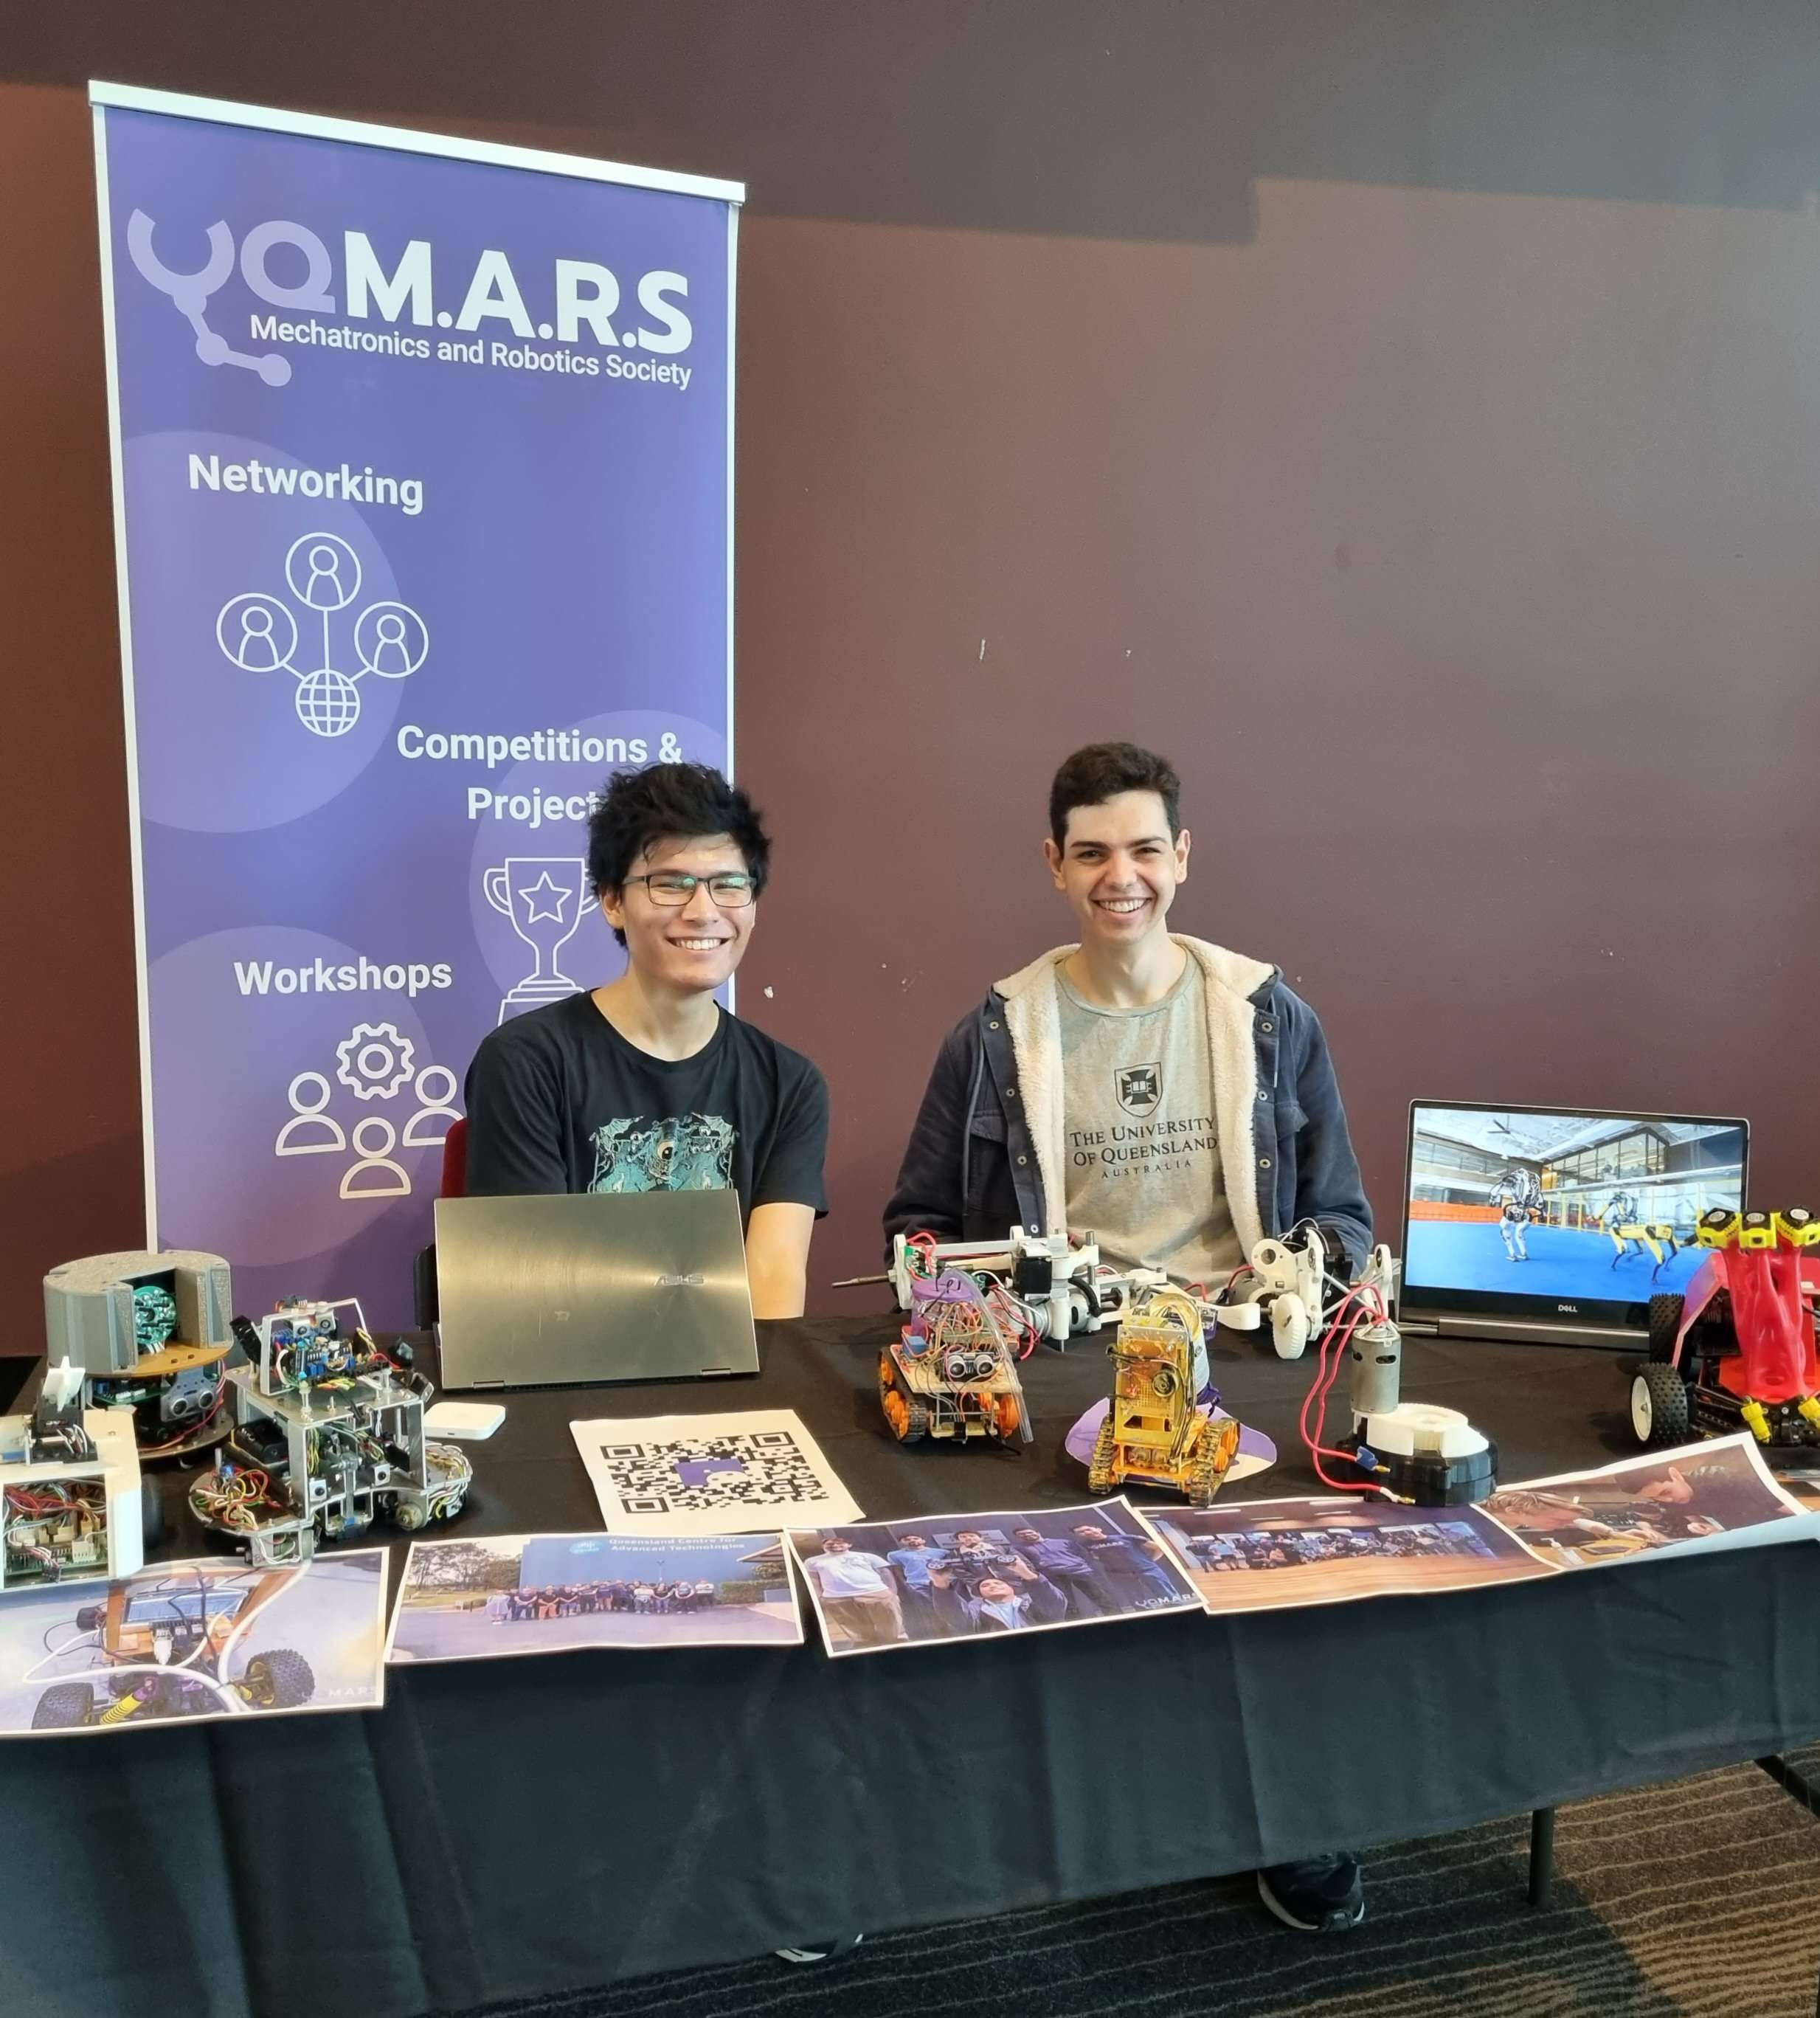
\includegraphics[width=0.99\linewidth]{prospectus/2024/Photos/2023Sem2EAITExpo1.jpg}
    \end{subfigure}
    \begin{subfigure}{0.32\linewidth}
        \includegraphics[width=0.99\linewidth]{prospectus/2024/Photos/Welcome-14.jpg}
    \end{subfigure}
\end{figure}

% ------------------------ INSERT IMAGE HERE ------------------------ %

\newpage

\section*{2023 In Review}

In 2023, UQMARS saw massive success, through a variety of events, collaborations, and an increase in membership numbers more than triple to 161 when compared to 2021 (with an average of approximately 20\% attendance at each event).
Some of our notable events in 2023 include:

\vspace{-1cm}

\subsection{Arduino Hackathon}
The Arduino Hackathon was a three-day event held at River City Labs in collaboration with QUT Robotics Club and Robogals, with a theme of ‘automation’. Guest judges for the event included the likes of Steve Baxter and representatives from robotics companies across Australia.   

% ------------------------ INSERT IMAGE HERE ------------------------ %
\begin{figure}[H]
    \centering
    \begin{subfigure}{0.32\linewidth}
        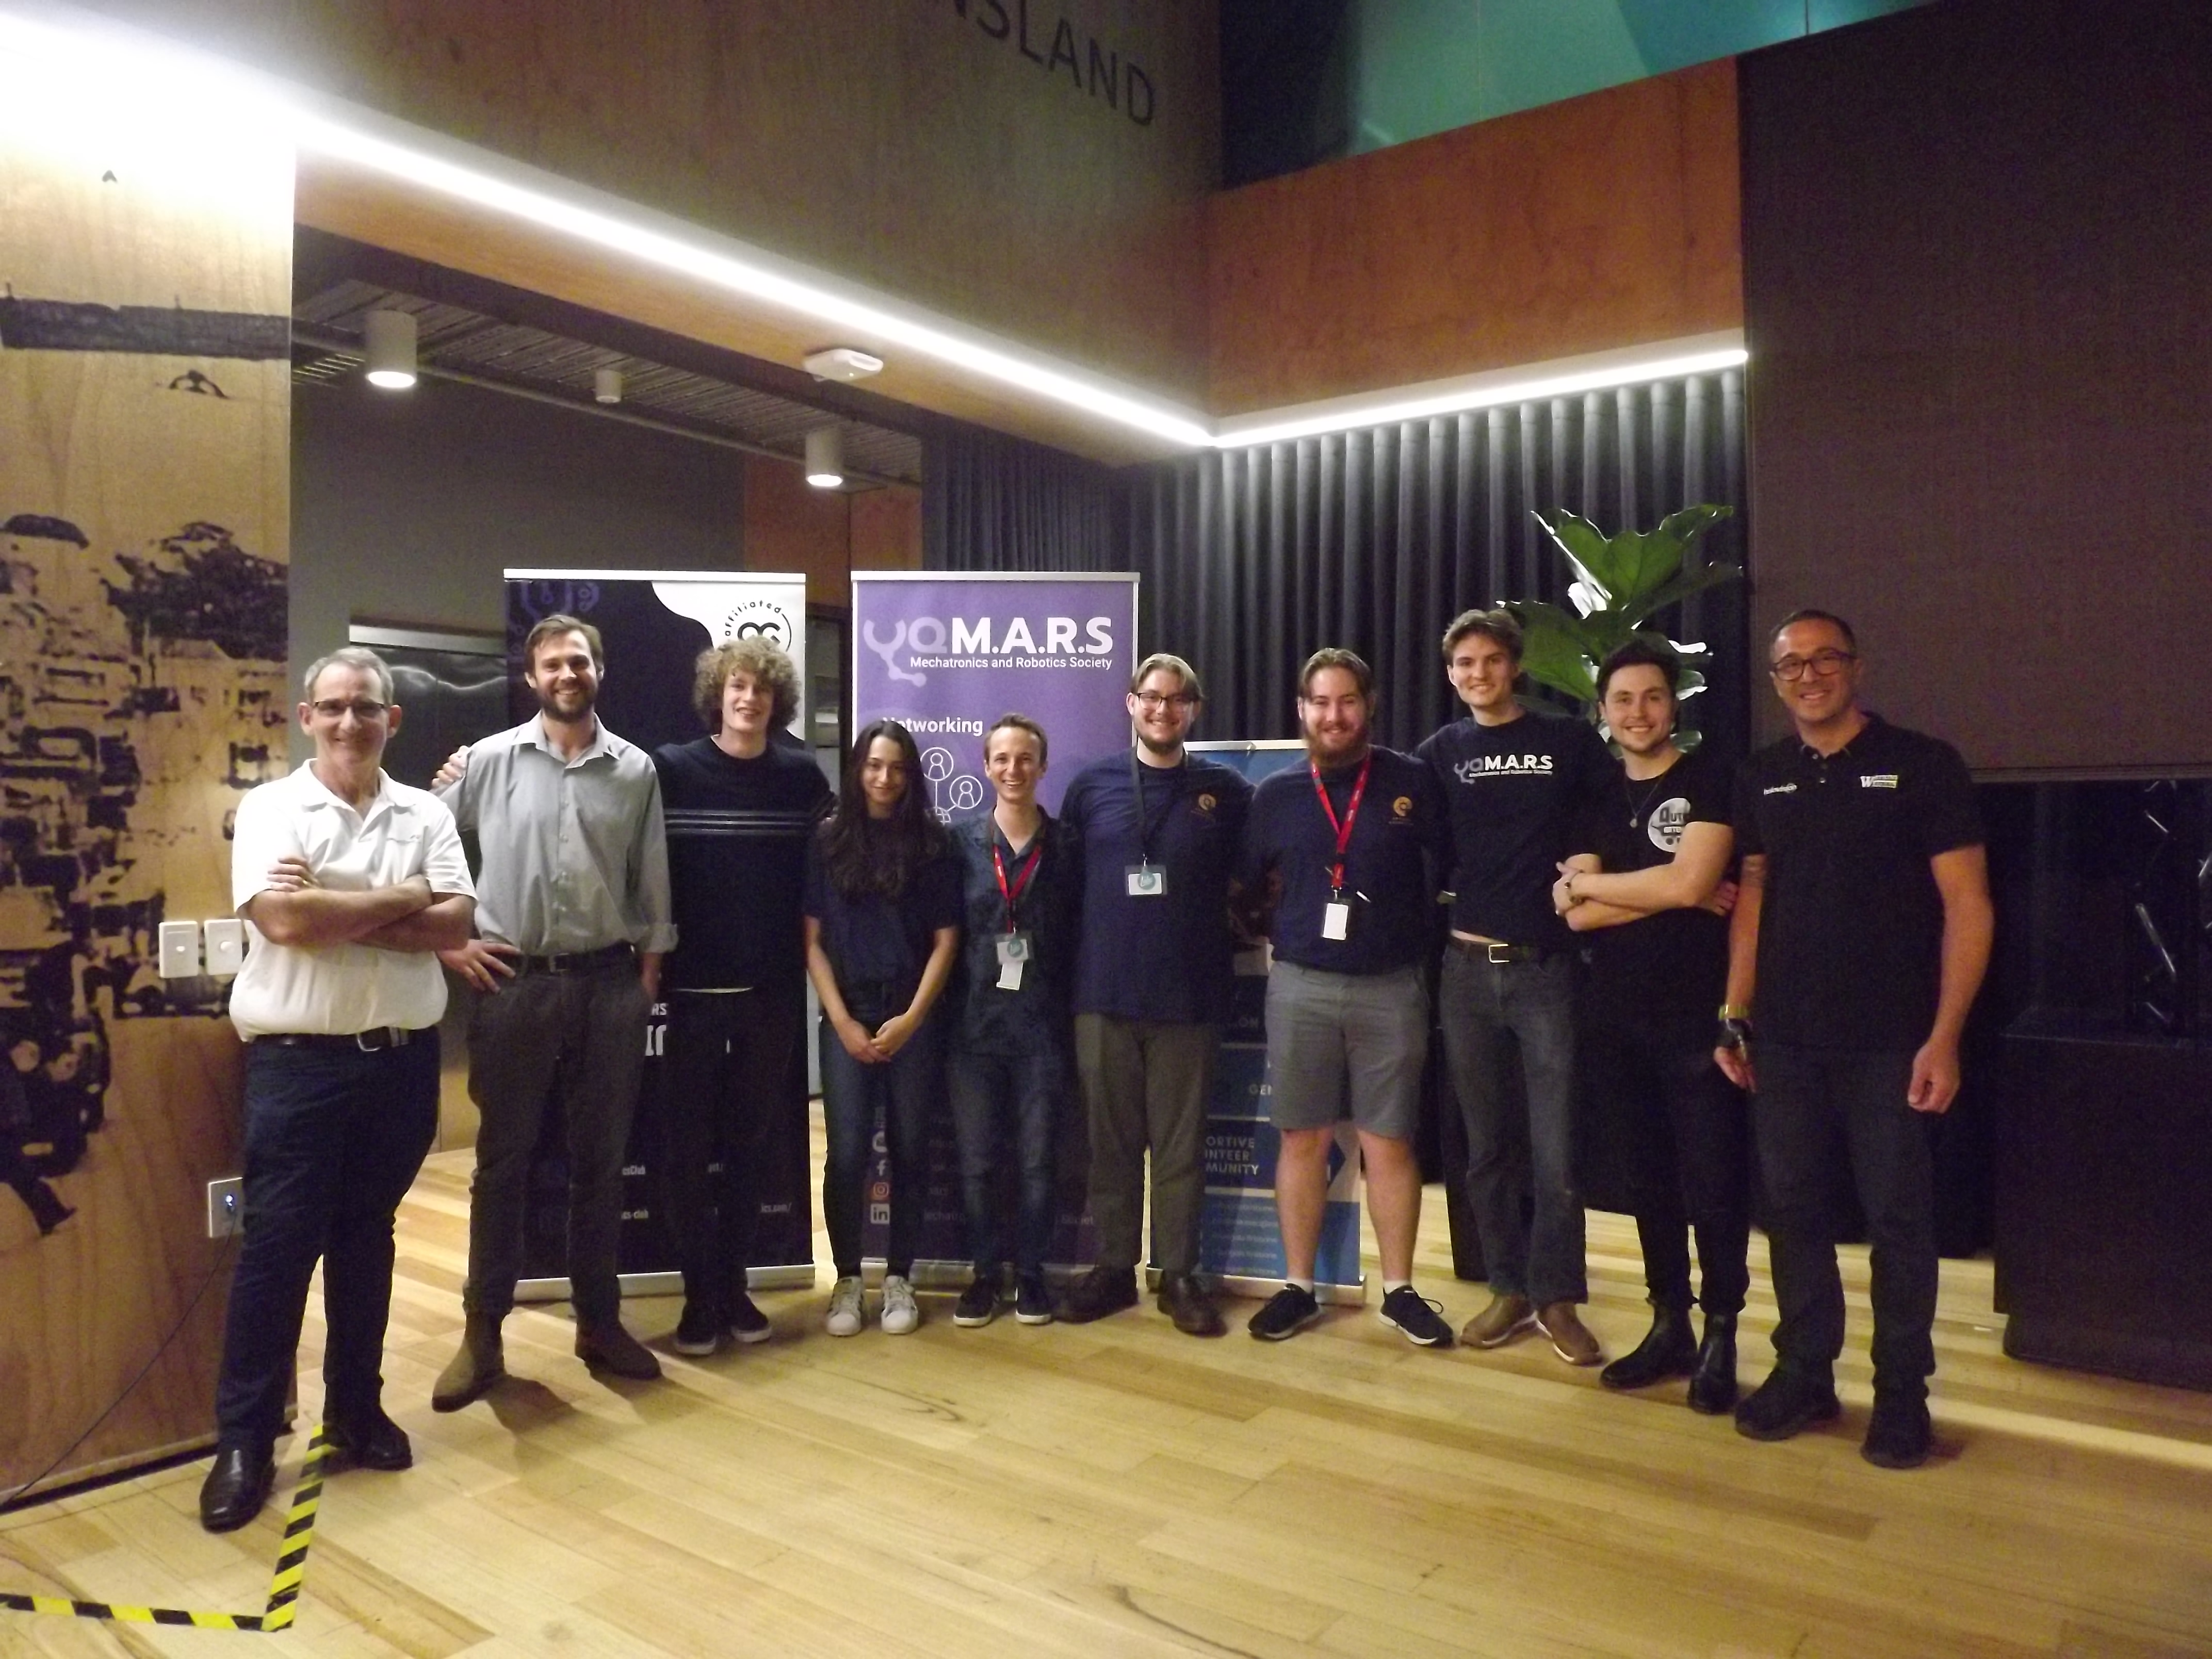
\includegraphics[width=0.99\linewidth]{prospectus/2024/Photos/ArdHackCombined.JPG}
    \end{subfigure}
    \begin{subfigure}{0.32\linewidth}
        \includegraphics[width=0.99\linewidth]{prospectus/2024/Photos/Arduino1.jpg}
    \end{subfigure}
    \begin{subfigure}{0.32\linewidth}
        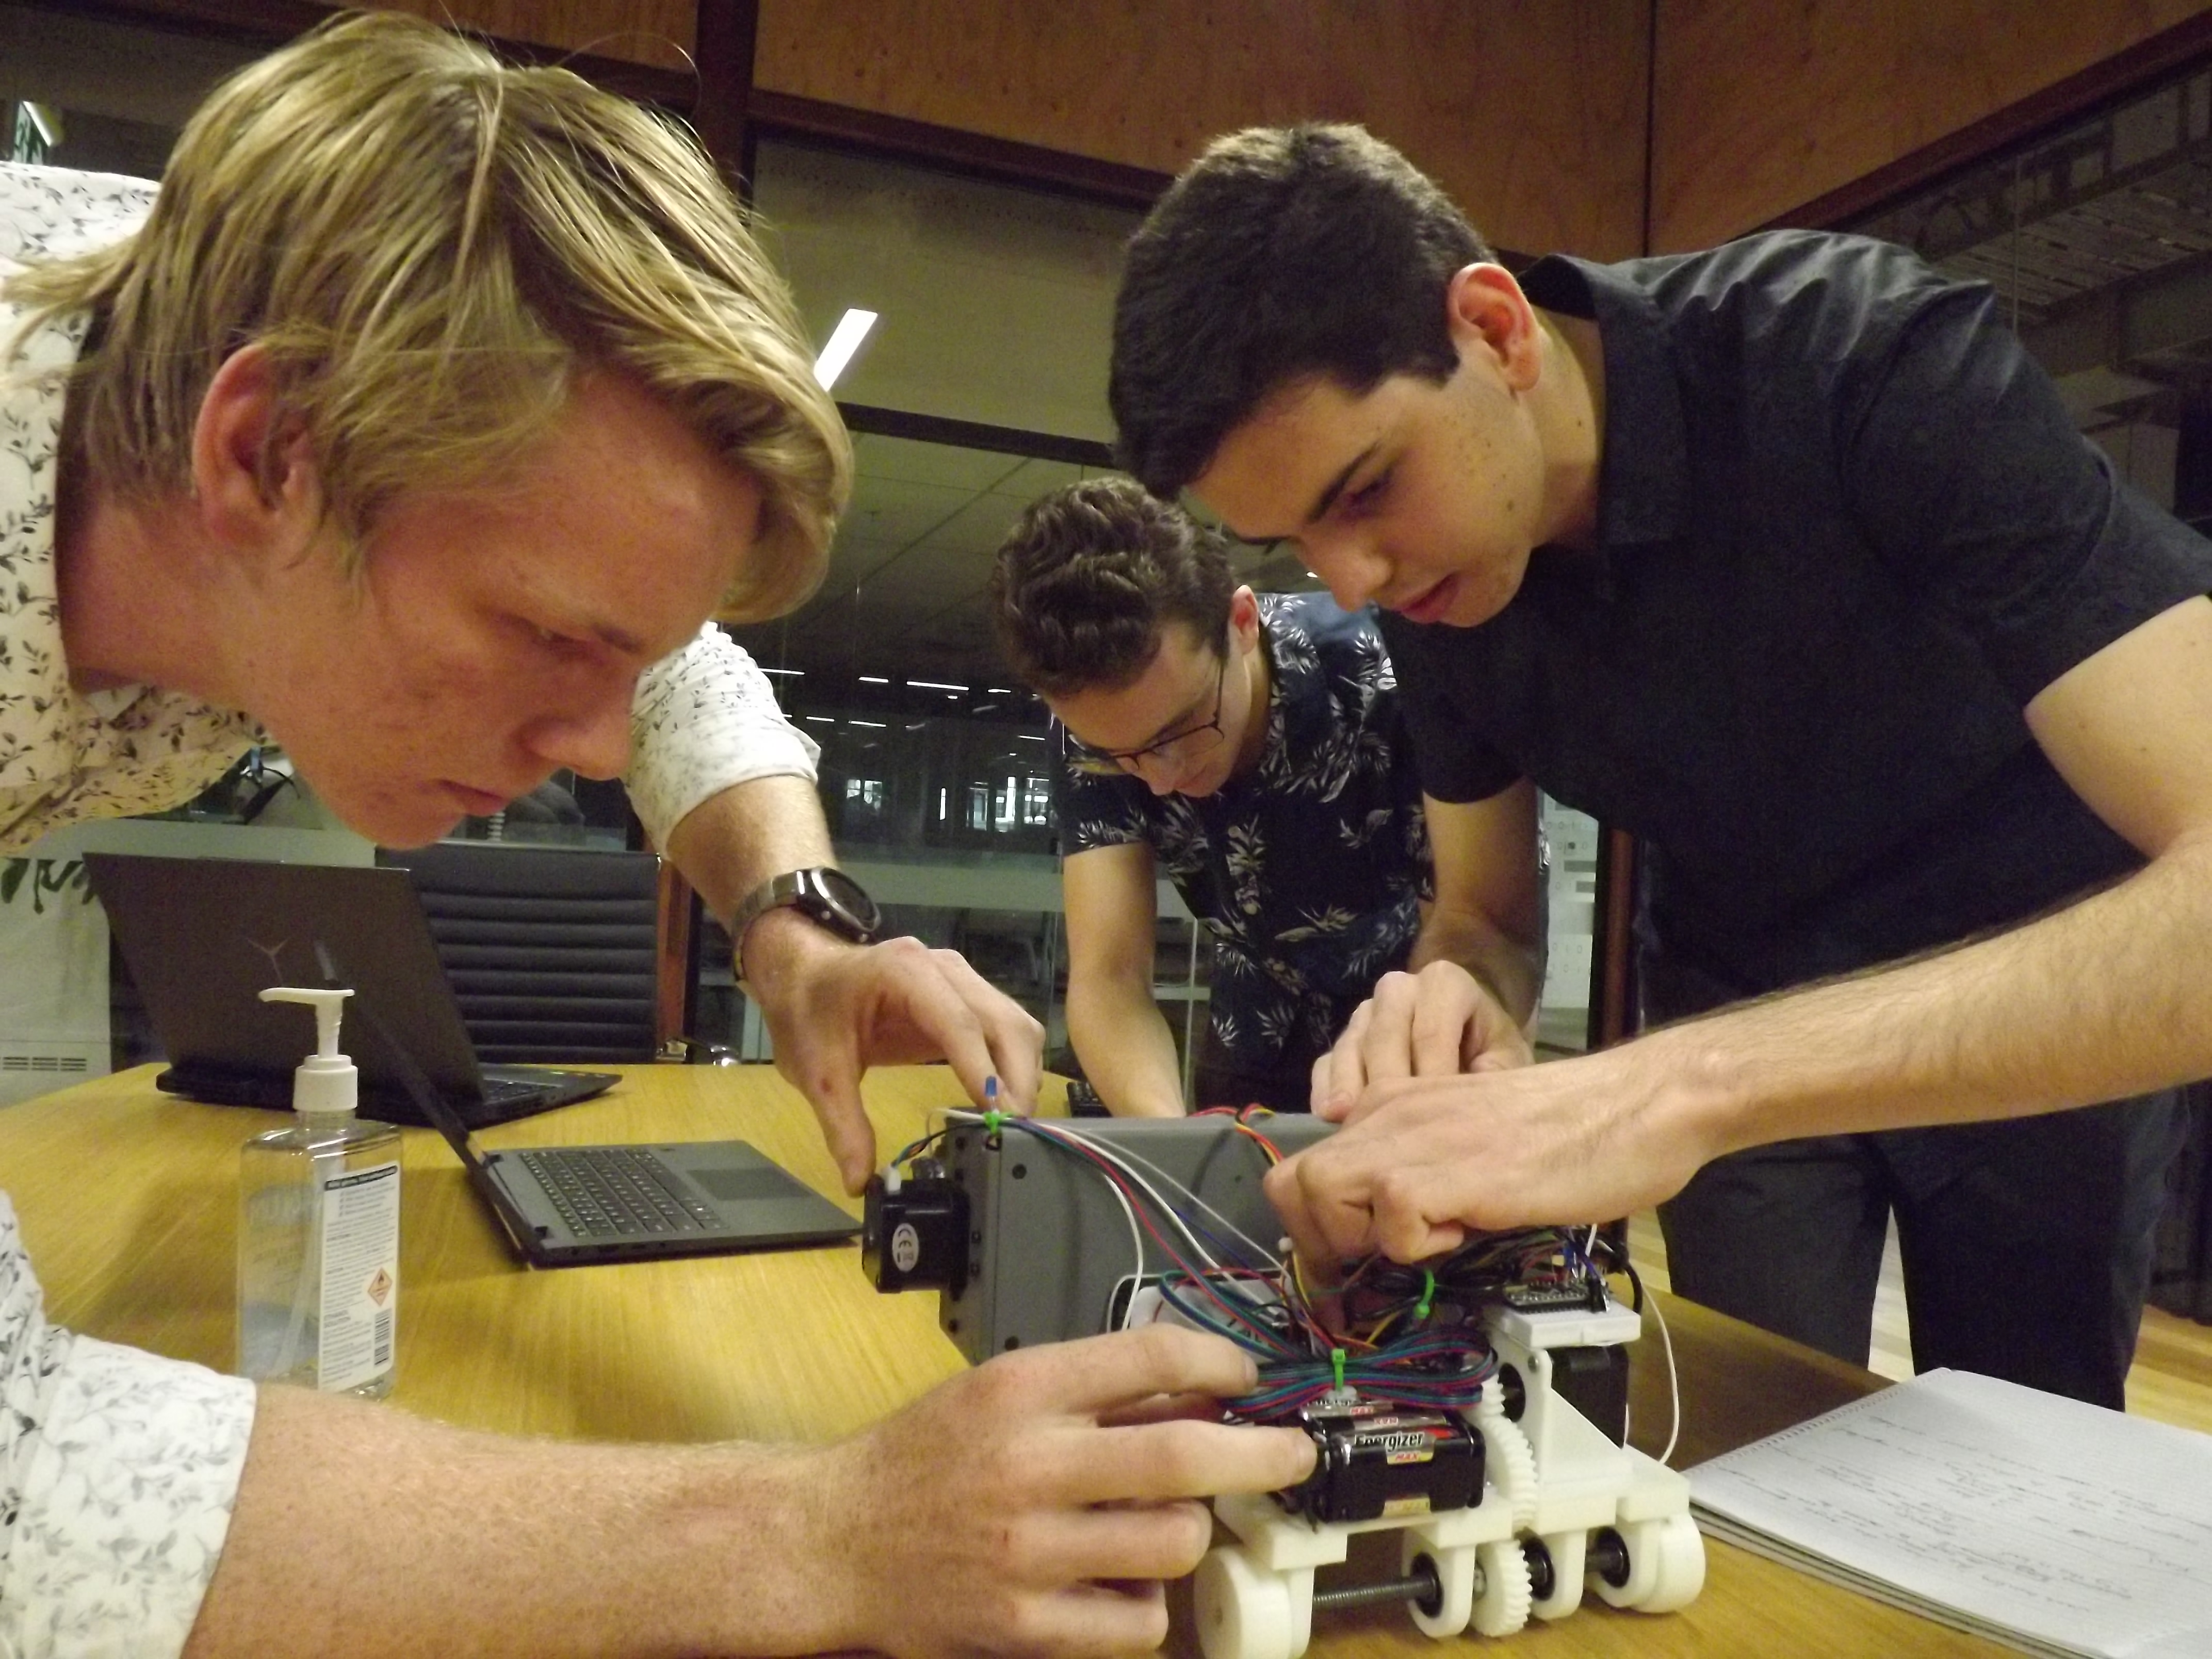
\includegraphics[width=0.99\linewidth]{prospectus/2024/Photos/winnerWinner.JPG}
    \end{subfigure}
\end{figure}

\vspace{-2cm}

\subsection{Mechatronics Panel Night}
This event was a collaboration with both QUT Robotics Club, Engineers Without Borders and Robogals and was designed to introduce members to applications of a mechatronic engineering degree, particularly through a humanitarian lens.
The evening featured professionals both from education and industry backgrounds to inspire members with their own experiences.

\vspace{-1.8cm}

\subsection{Droid Race Competition}
In 2023, UQ MARS entered two teams into the QUT Droid Race Challenge.
The competition presents an opportunity for members to get hands-on experience with computer vision, control systems, and mechanical design.
Teams performed admirably, with both managing to outperform the hosts and one team winning the Organisers Choice Award.
The event served as an opportunity for members to test their abilities and develop new skills around developing with embedded systems. 
\begin{figure}[H]
    \centering
    \begin{subfigure}{0.32\linewidth}
        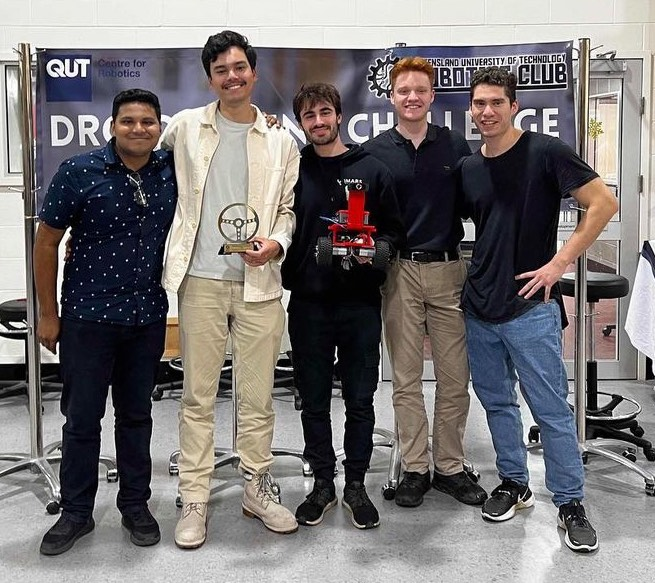
\includegraphics[width=0.99\linewidth]{prospectus/2024/Photos/DRC_EXECTEAM.jpg}
    \end{subfigure}
    \begin{subfigure}{0.32\linewidth}
        \includegraphics[width=0.99\linewidth]{prospectus/2024/Photos/PCB-03.jpg}
    \end{subfigure}
    \begin{subfigure}{0.32\linewidth}
        \includegraphics[width=0.99\linewidth]{prospectus/2024/Photos/CAD-5.jpg}
    \end{subfigure}
\end{figure}

\vspace{-1.8cm}

\subsection{UQ MARS Outreach Program}
In conjunction with the University EAIT Department planned and presented a workshop on working with Arduino's tailored to a high school level curriculum, this event was successful and laid the groundwork to an ongoing workshop series for schools around the city that wish to introduce their students to the field of Mechatronics at an early age.

\vspace{-1.8cm}

\subsection{MARS Workshop Series}
One of our most successful events of the year was our workshop series. This included the likes of our Mechanical CAD, PCB, Computer Vision, Path-planning and ROS2 Workshops all lead by both Executives and Graduates respectively.

\vspace{-1.5cm}

\subsection{Networking Night} 
Our annual Networking Night held at River City Labs was an opportunity for our members to interact with representatives from industry and academia alike.
% ------------------------ INSERT IMAGE HERE ------------------------ %
\begin{figure}[H]
    \centering
    \begin{subfigure}{0.42\linewidth}
        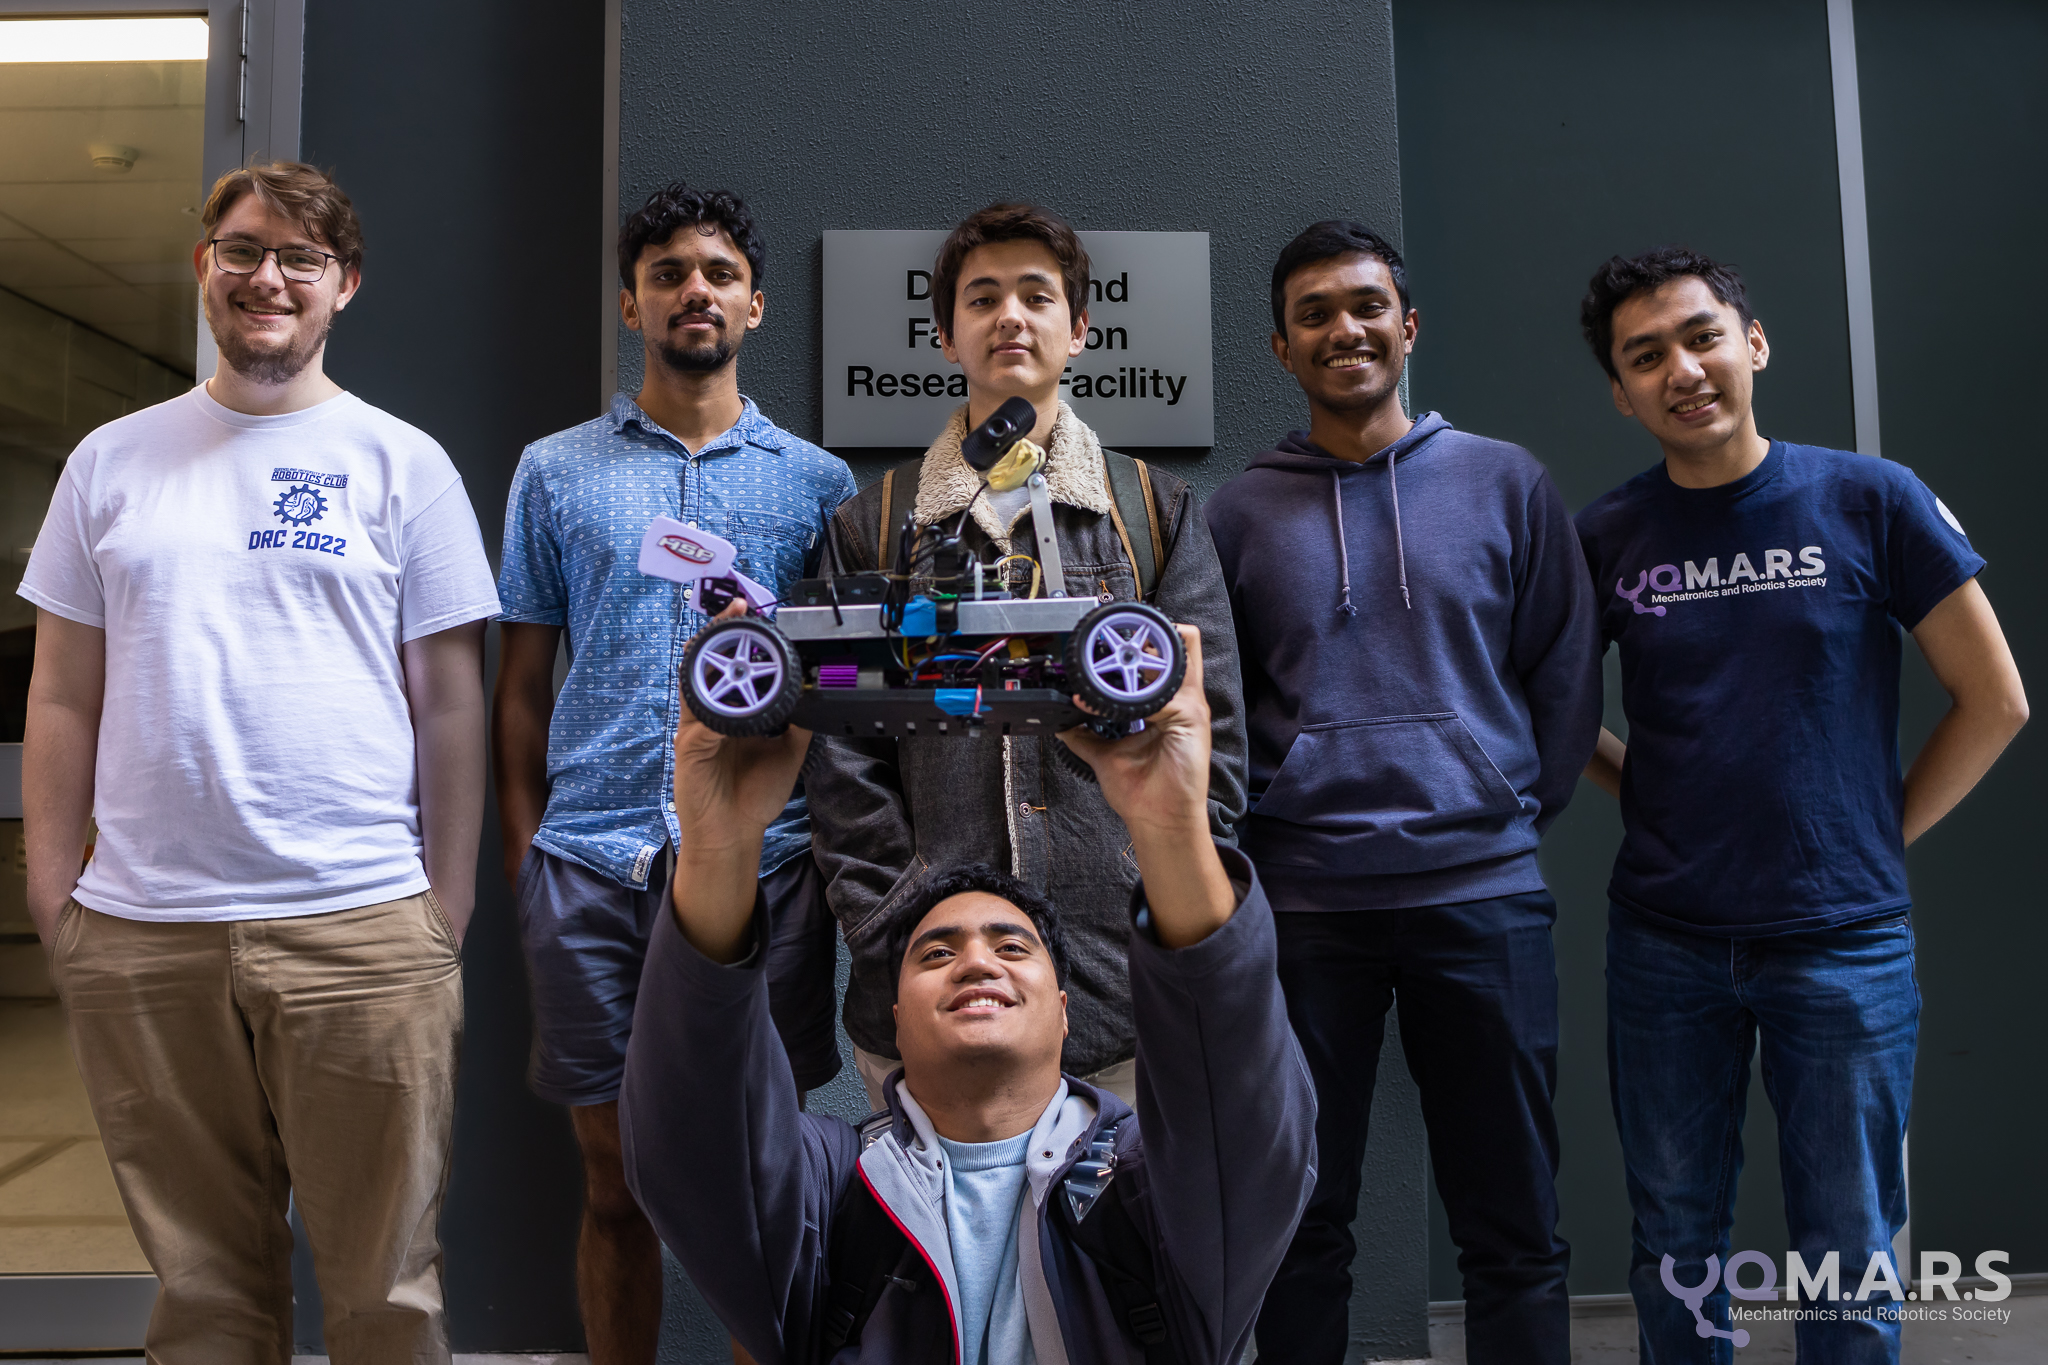
\includegraphics[width=0.99\linewidth]{prospectus/2023/Photos/DRC.jpg}
    \end{subfigure}
    \begin{subfigure}{0.42\linewidth}
        \includegraphics[width=0.99\linewidth]{prospectus/2023/Photos/CSIRO.jpg}
    \end{subfigure}
\end{figure}
\newpage

\subsection{Micromouse Competition} 
 In 2023 UQ MARS held out inaugural micromouse competition that saw teams from different universities and disciplines compete.
% ------------------------ INSERT IMAGE HERE ------------------------ %
\begin{figure}[H]
    \centering
    \begin{subfigure}{0.32\linewidth}
        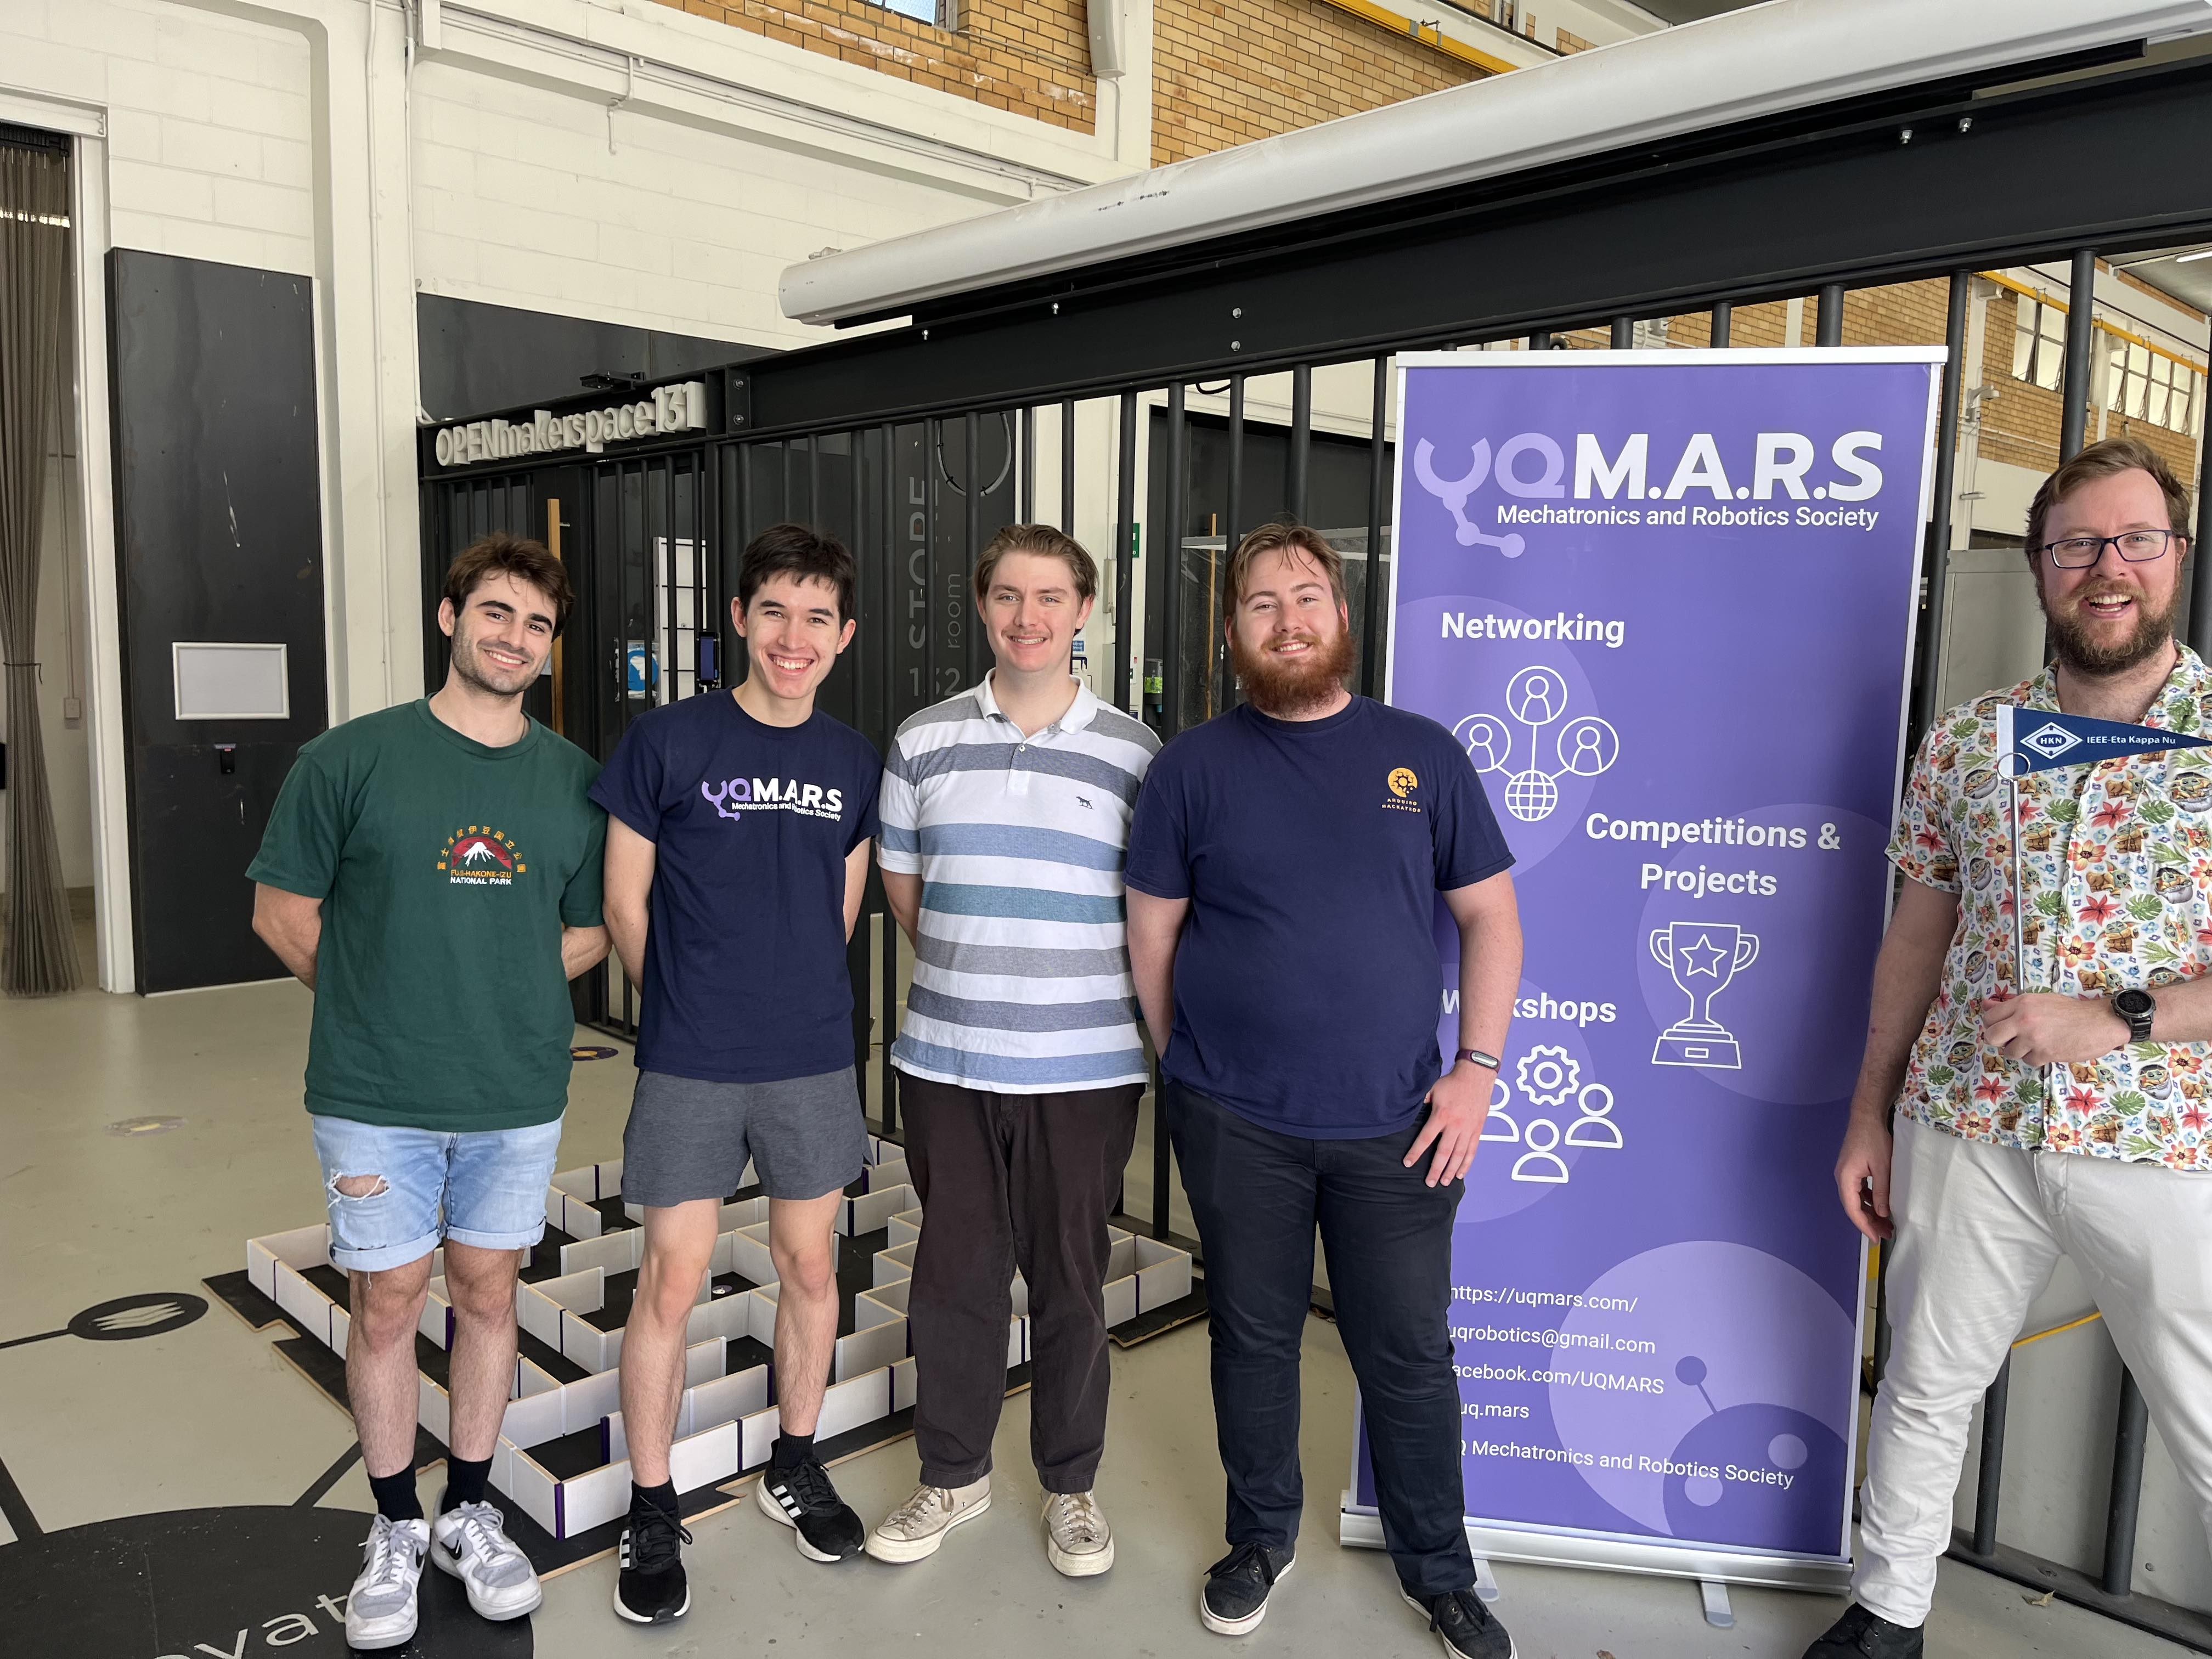
\includegraphics[width=0.99\linewidth]{prospectus/2024/Photos/ExecMouse.jpg}
    \end{subfigure}
    \begin{subfigure}{0.32\linewidth}
        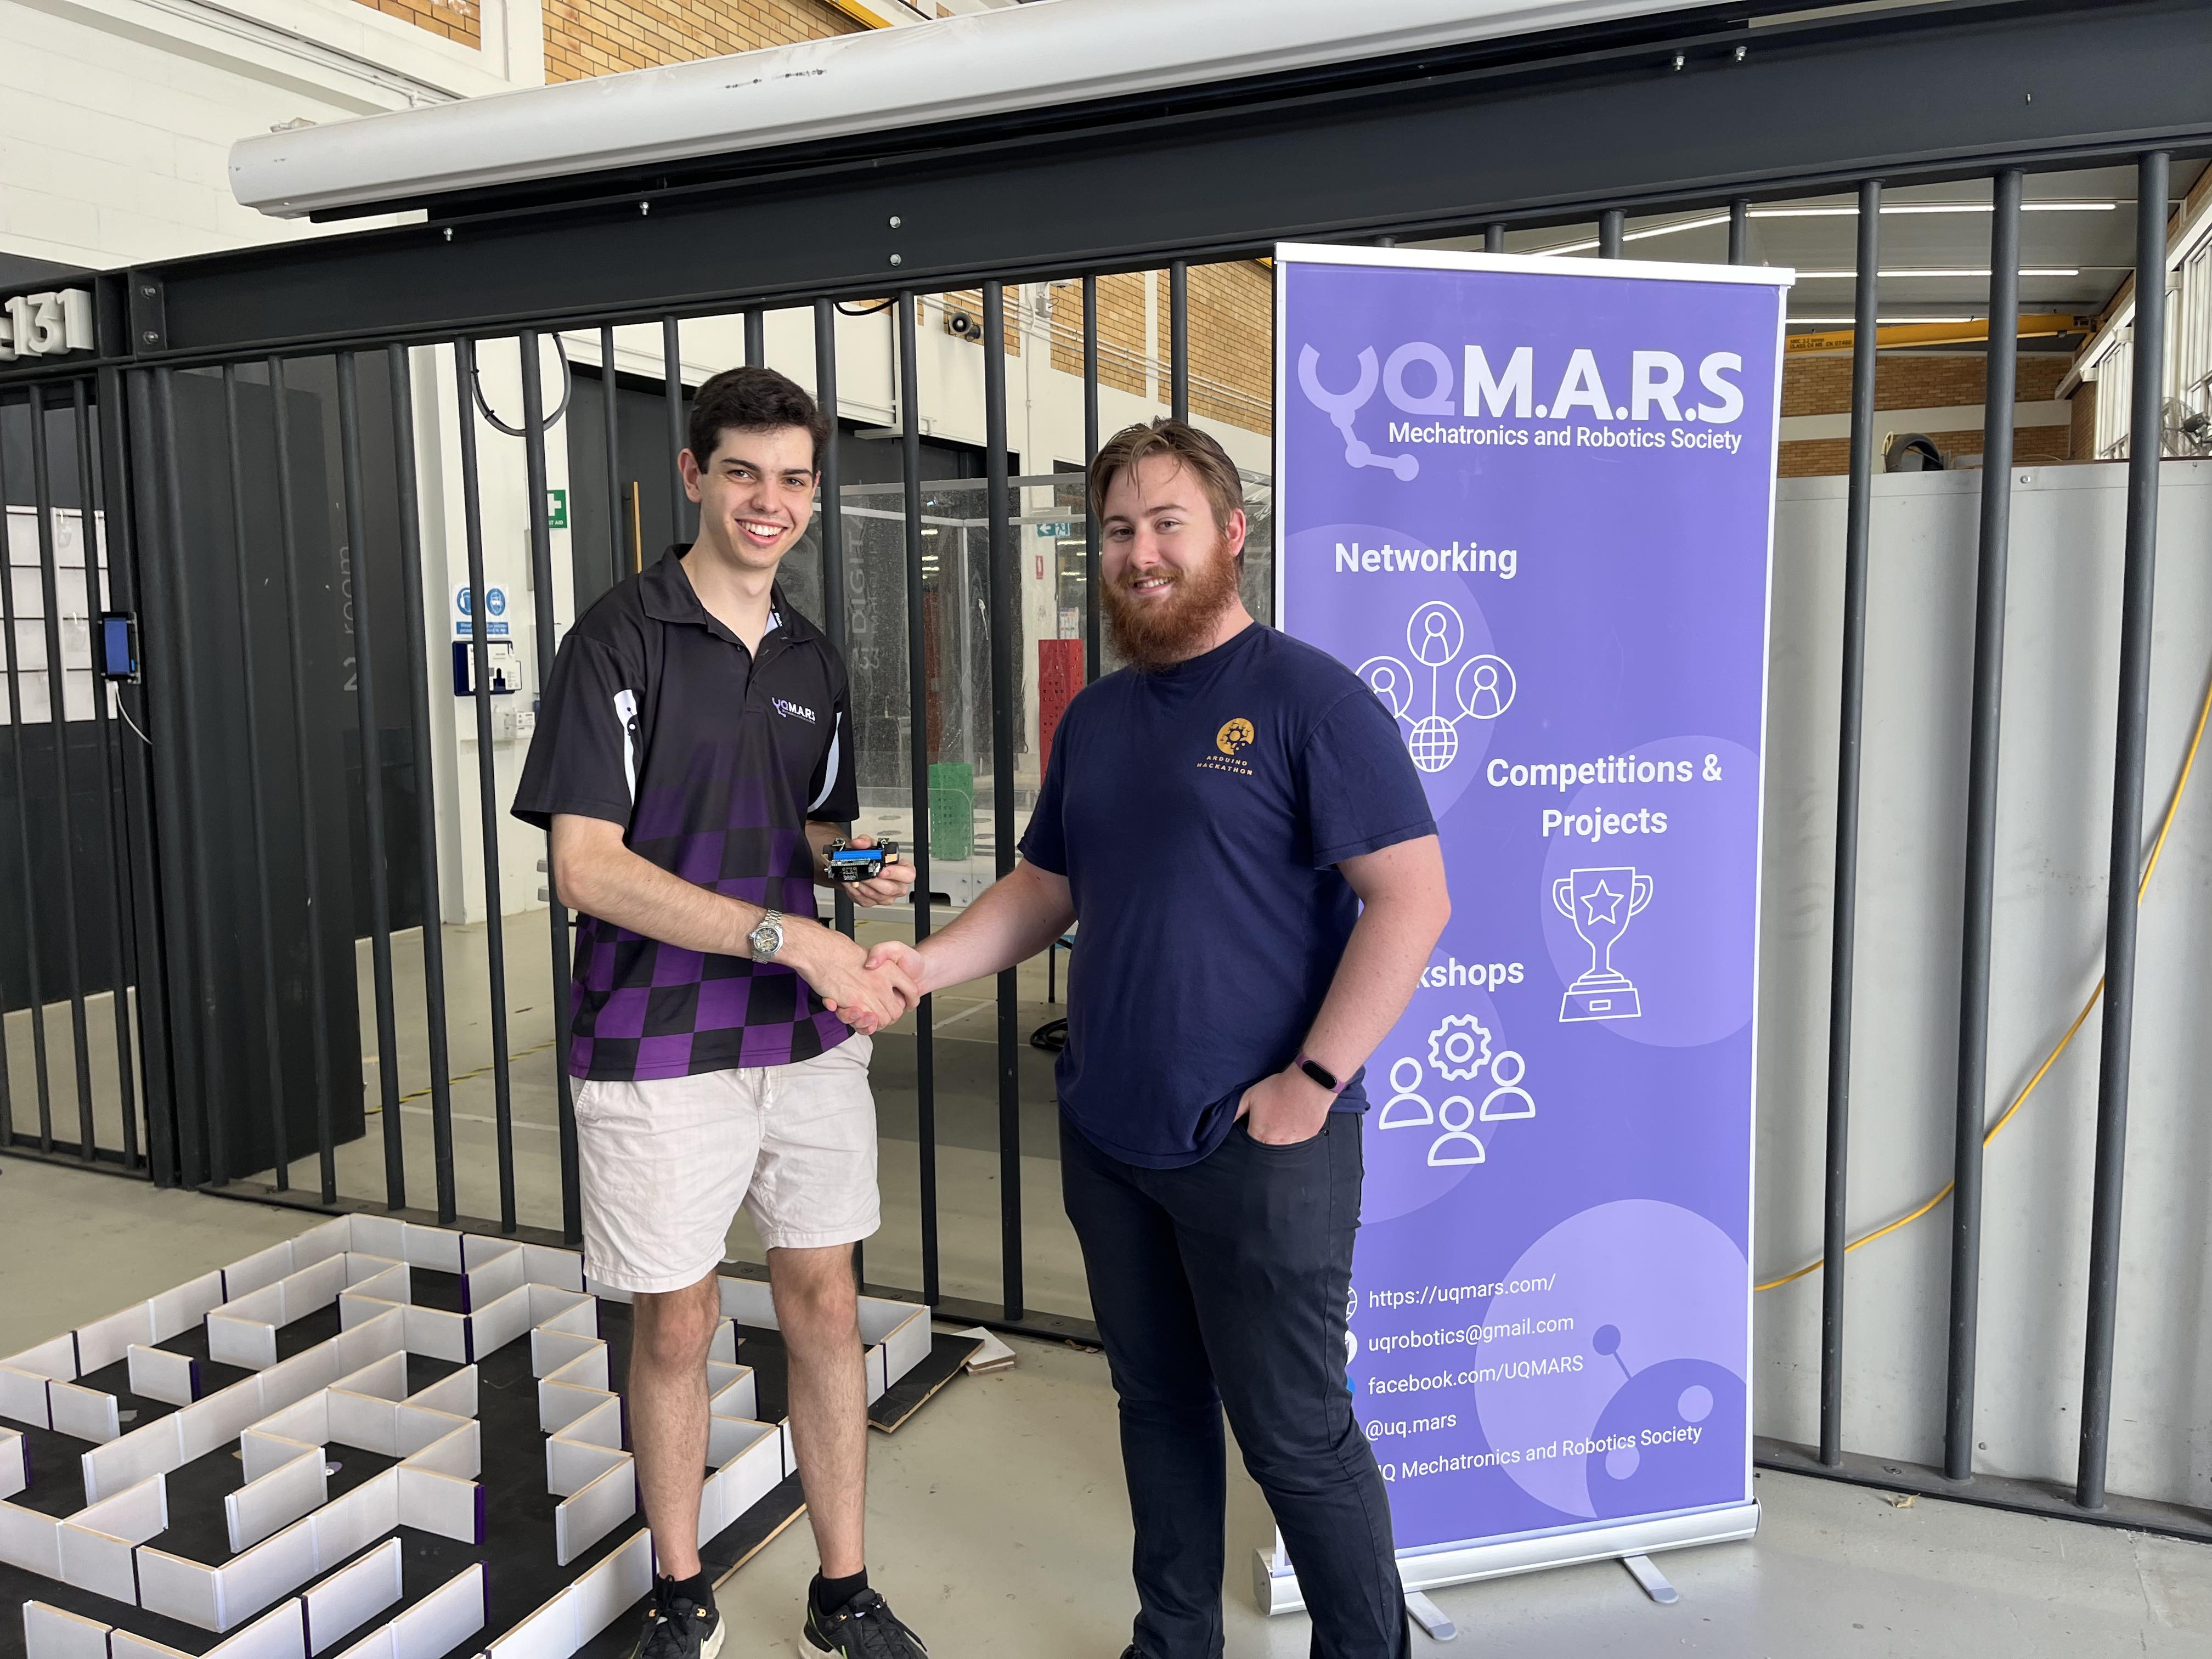
\includegraphics[width=0.99\linewidth]{prospectus/2024/Photos/Goat.jpg}
    \end{subfigure}
    \begin{subfigure}{0.32\linewidth}
        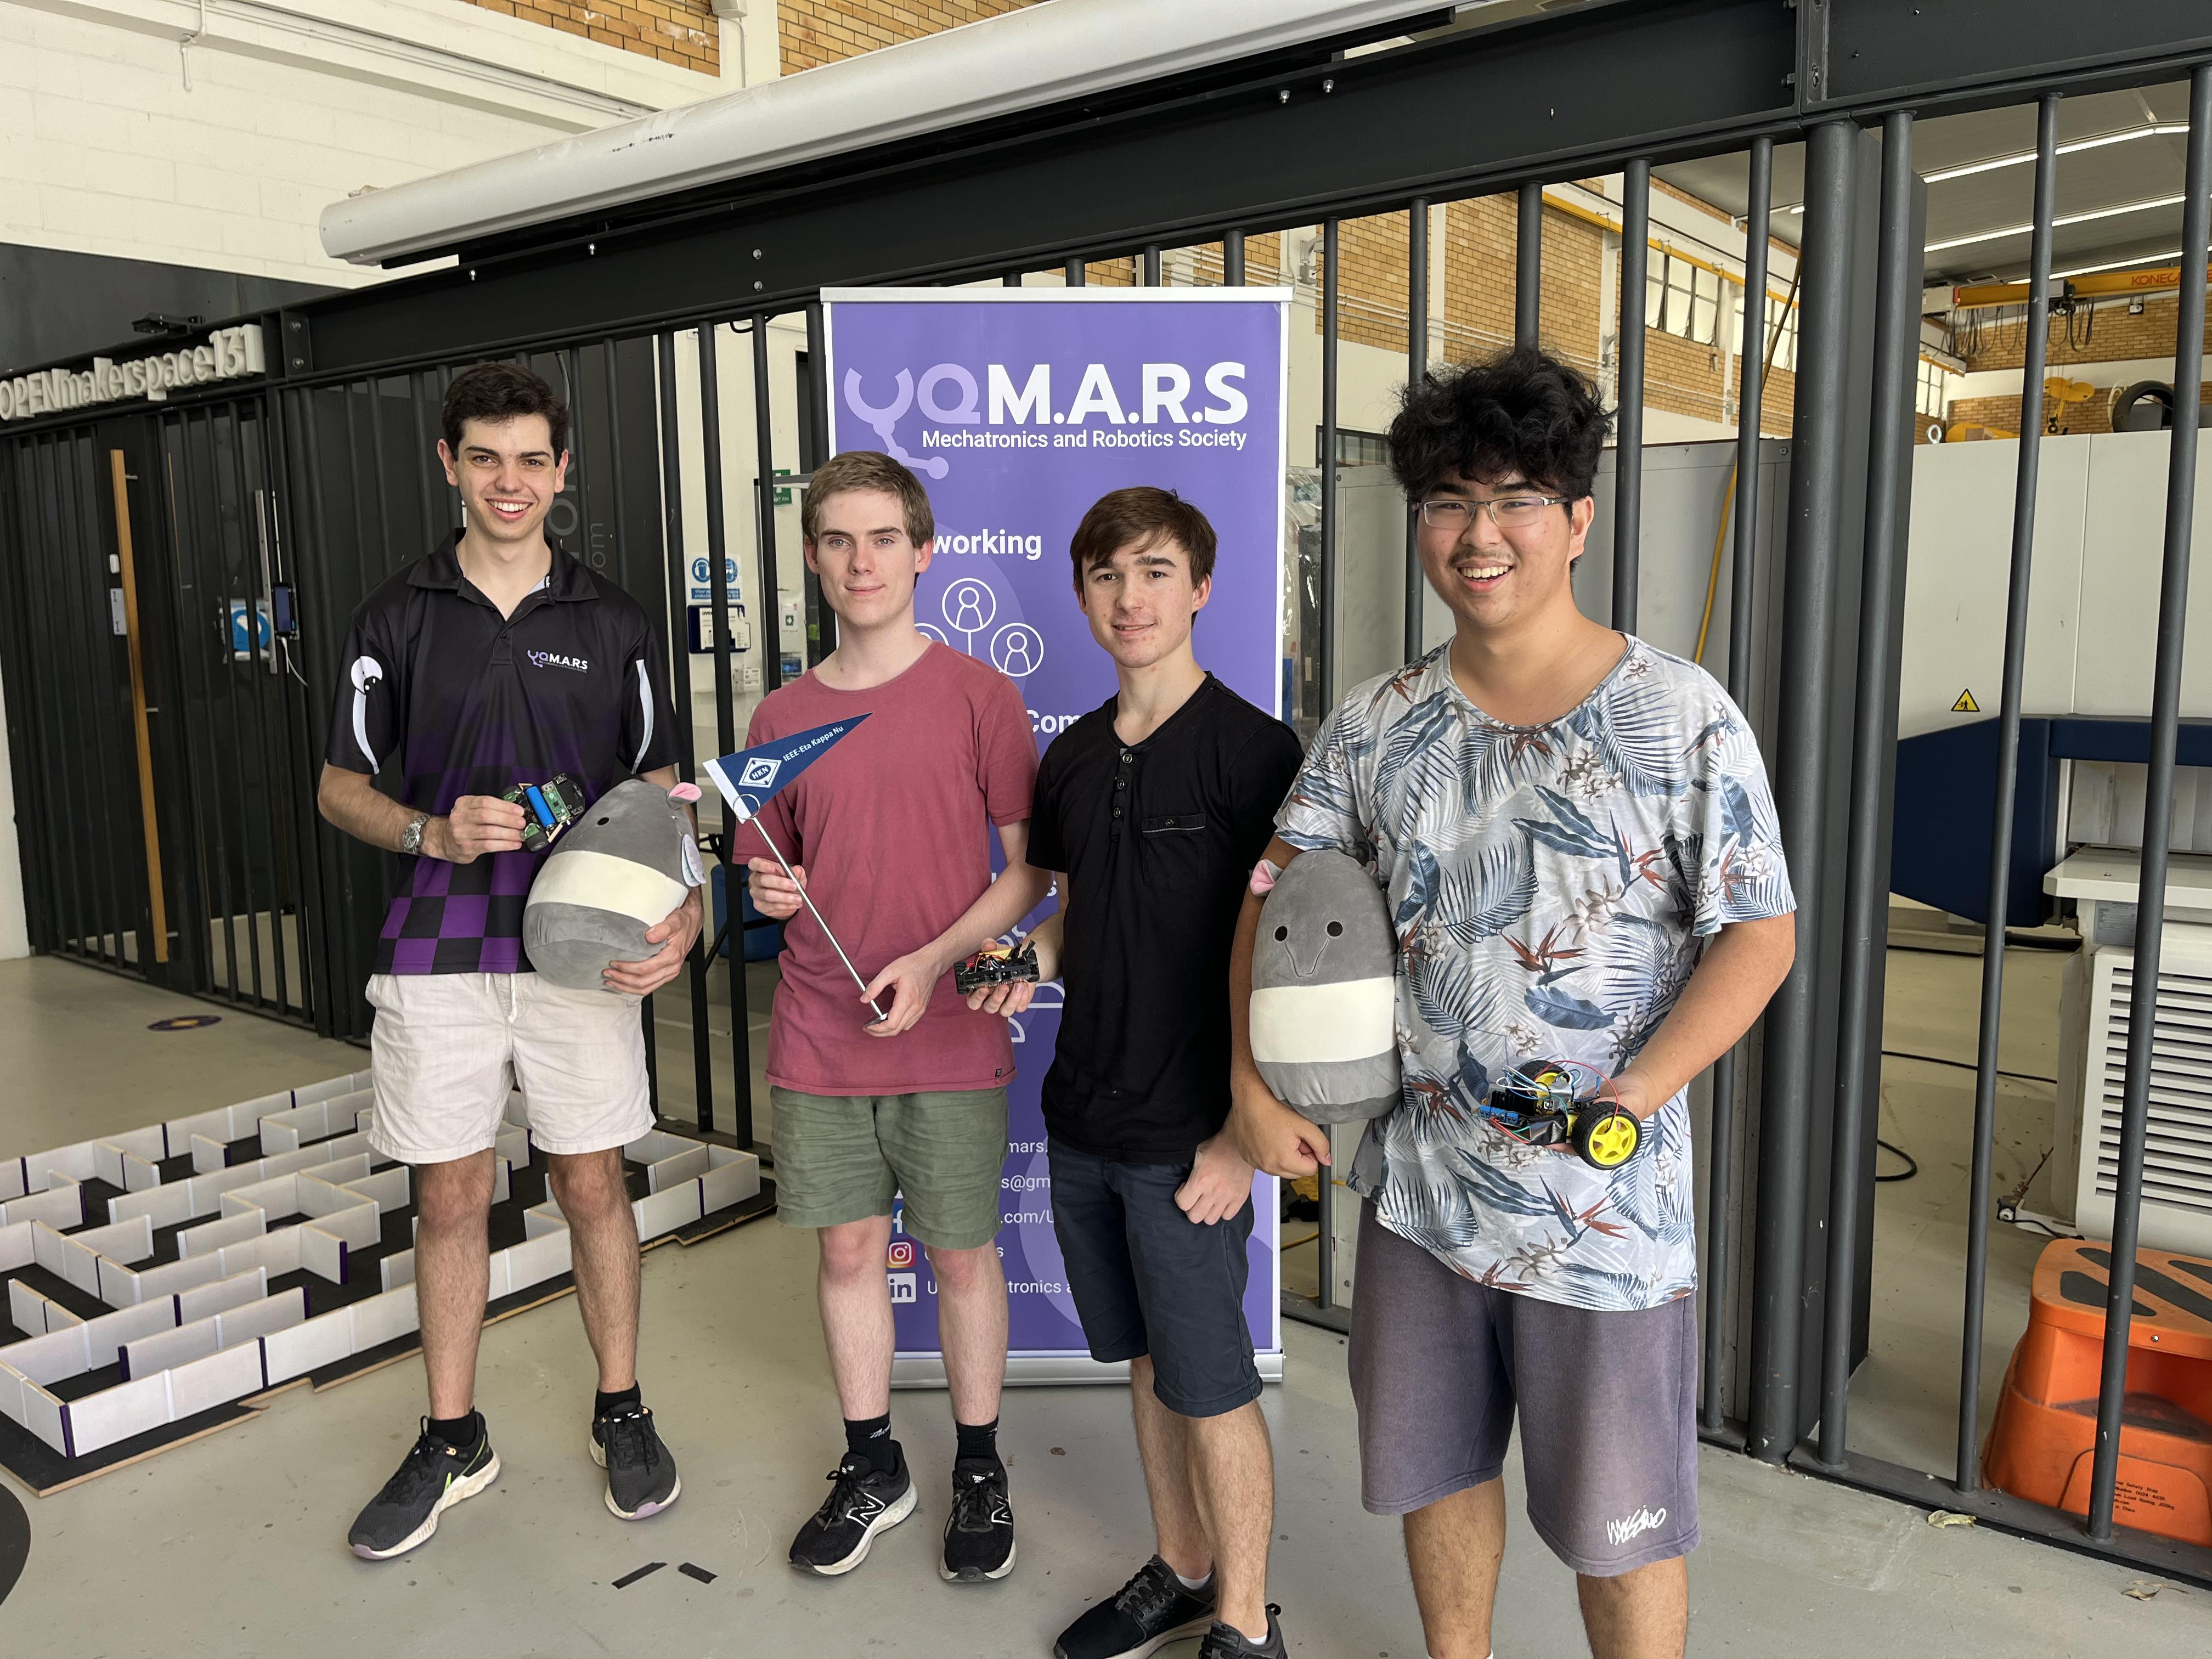
\includegraphics[width=0.99\linewidth]{prospectus/2024/Photos/MouseWinners.jpg}
    \end{subfigure}
\end{figure}

\begin{figure}[H]
    \centering
    \begin{subfigure}{0.32\linewidth}
        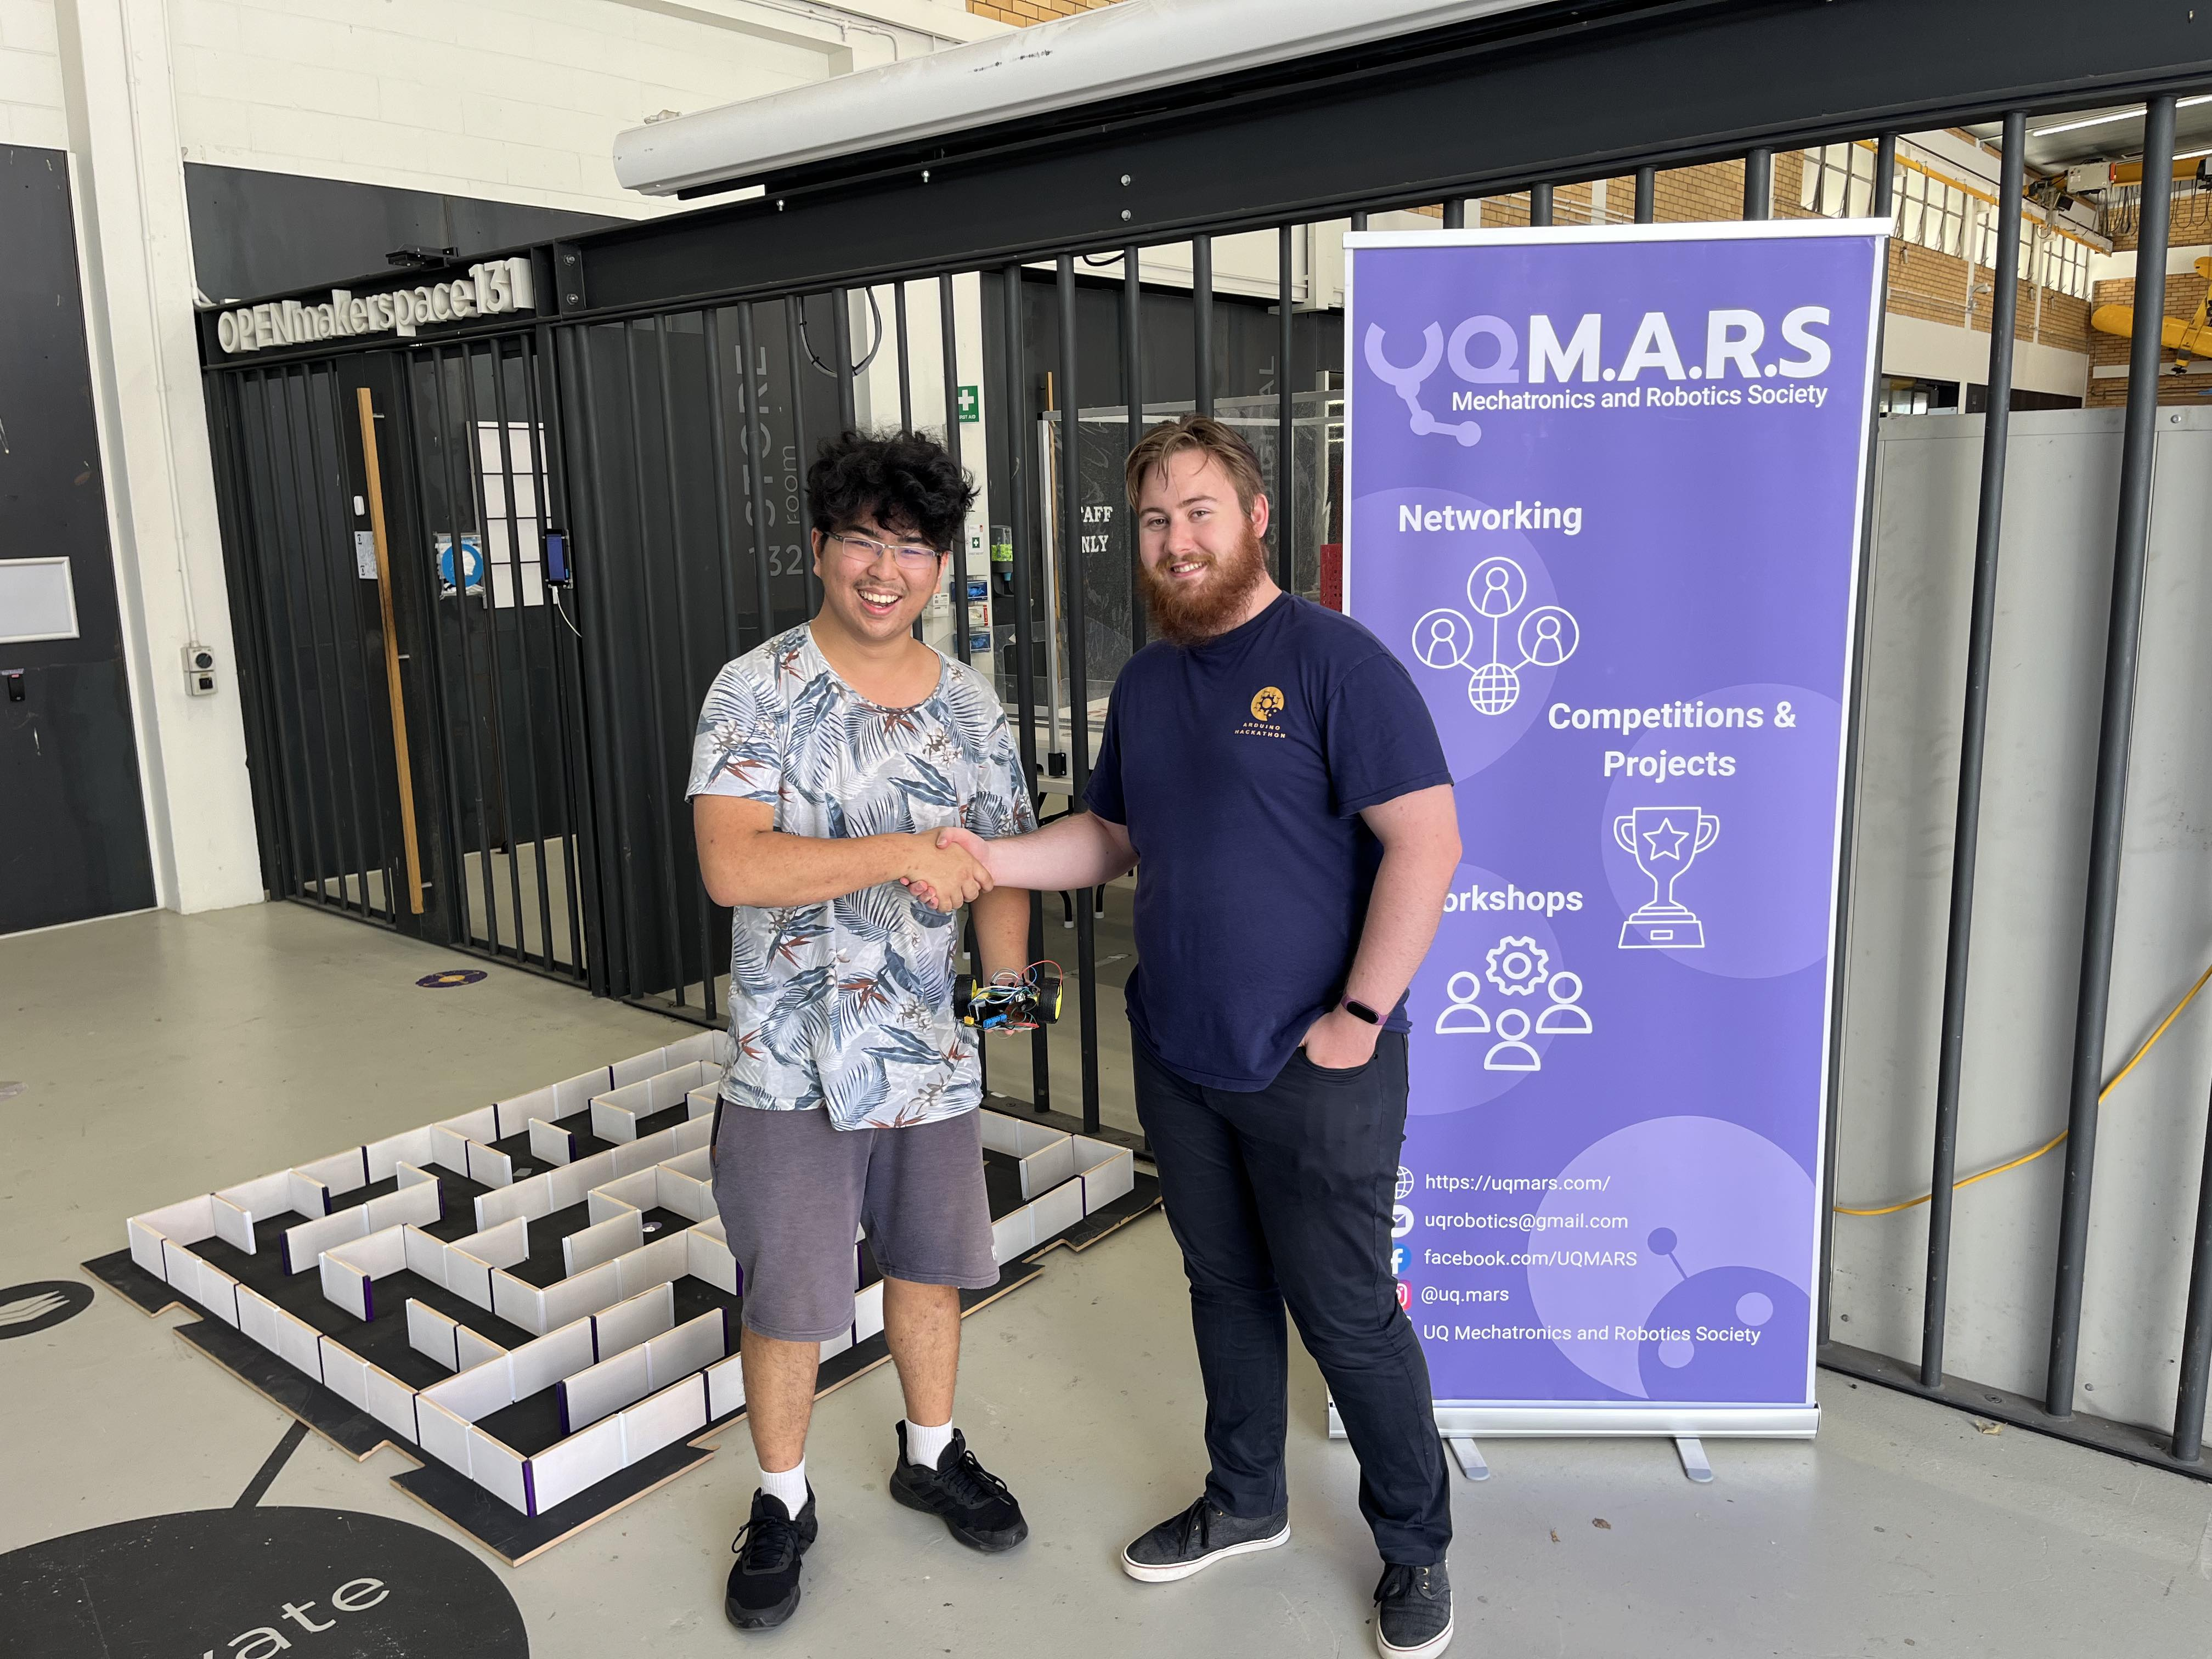
\includegraphics[width=0.99\linewidth]{prospectus/2024/Photos/SecondPlace.jpg}
    \end{subfigure}
    \begin{subfigure}{0.32\linewidth}
        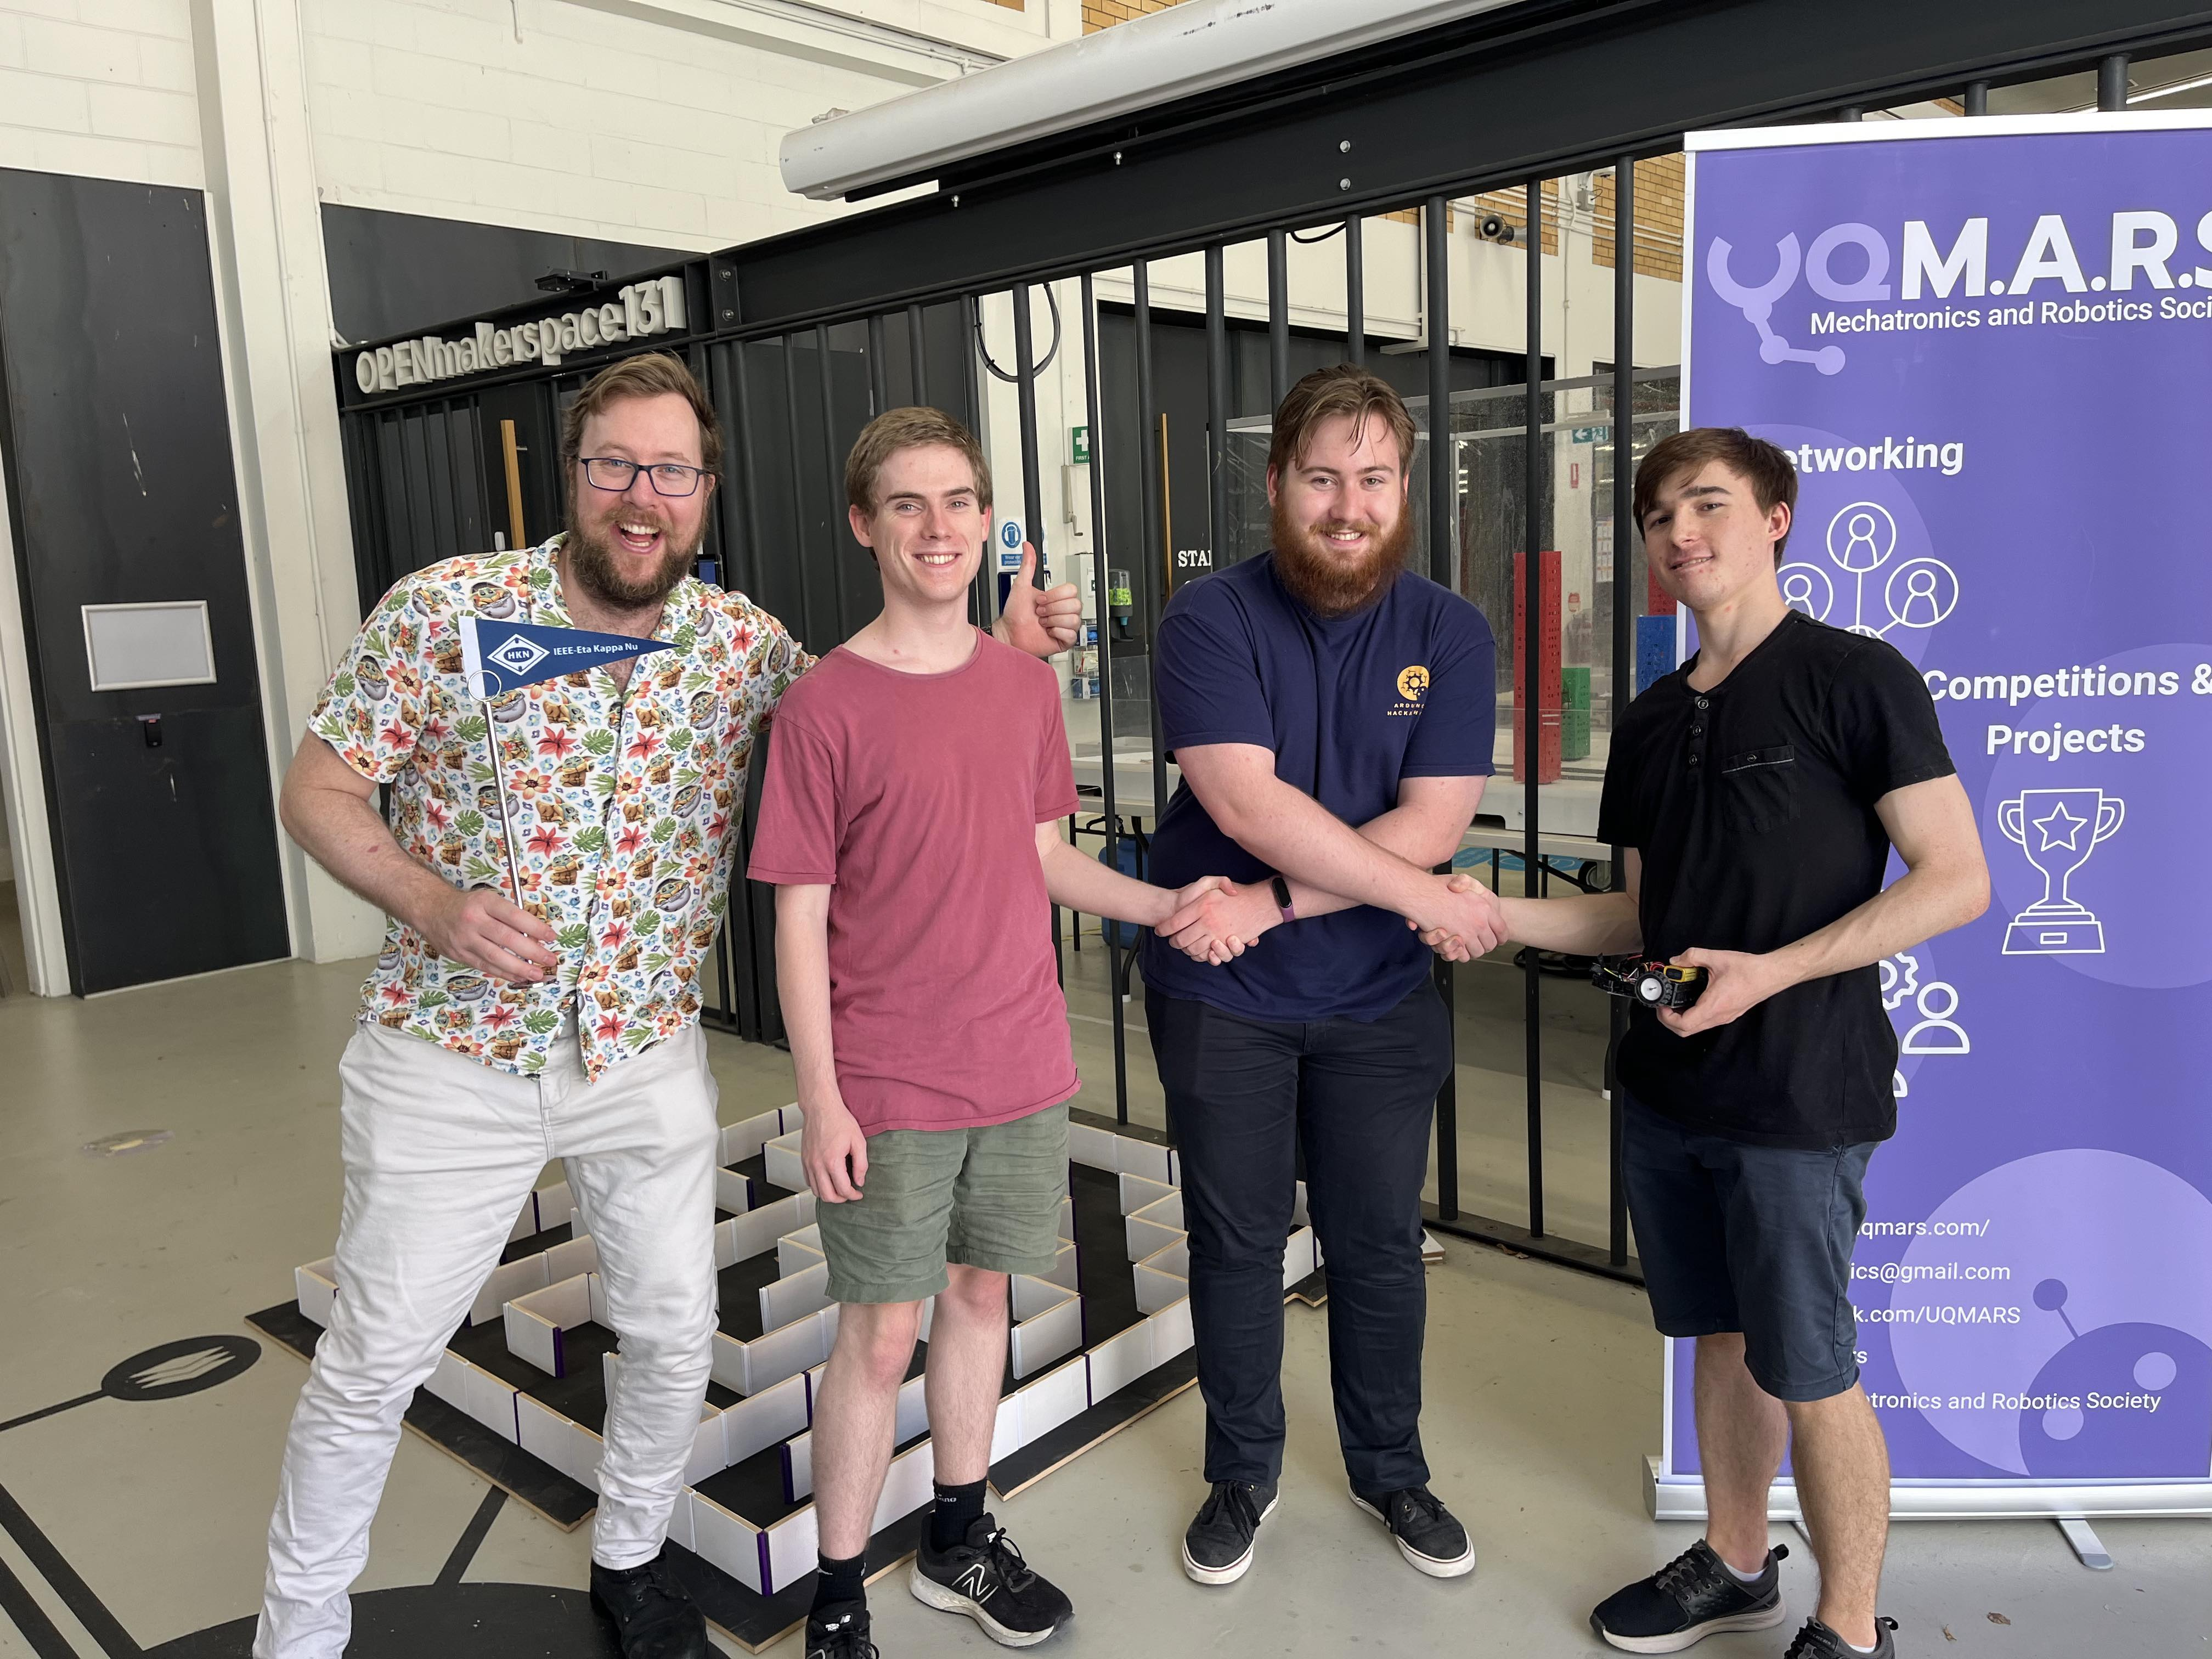
\includegraphics[width=0.99\linewidth]{prospectus/2024/Photos/TeamSpiritz.jpg}
    \end{subfigure}
\end{figure}

\vspace{-1.5cm}

\subsection{For our Partners}
What sets UQ MARS apart from other societies is our freedom to hold events alongside neighbouring societies and universities therefore our outreach is not only greatly beneficial to our members but also our partners as a partner of MARS is known throughout the academic space across Brisbane.

In 2023 we successfully held over 20 events that ranged from social events to hackathons, in 2024 we hope to extend this with more partnership engagement. Especially within our workshop series which includes the use of many different CAD software as well as simulation software. When it comes to skills we have taught over the year our members gained exposure to the following but not limited to:
\begin{itemize}
    \item Audesk Inventor
    \item Altium Designer
    \item Python Open CV
    \item ROS2 Humble
\end{itemize}

%% End Update Section ------------------------------------------------------------------------------------
\newpage

\section*{UQ MARS in 2024}
\subsection*{Goals}
After achieving positive growth in both members and events in 2023 we are looking ahead to 2024, UQ MARS is focused on building on past achievements as a foundation from which we can grow. Having a successful 2023 in 2024 we hope to expand on:
% Update this Section ------------------------------------------------------------------------------------
\begin{itemize}
    \item Advancing member experience
    \item Increase the amount of Mechatronics 
    \item Provide more opportunities for members to develop essential mechatronics skills
    \item Build industry connections and collaborations
    \item Drive the social culture around the club
    \item Give back to our community
\end{itemize}
% End Section ------------------------------------------------------------------------------------
% Add New photos ------------------------------------------------------------------------------------
\begin{figure}[H]
    \centering
    \begin{subfigure}{0.32\linewidth}
        \includegraphics[width=0.99\linewidth]{Photos/Hackathon.jpg}
    \end{subfigure}
    \begin{subfigure}{0.32\linewidth}
        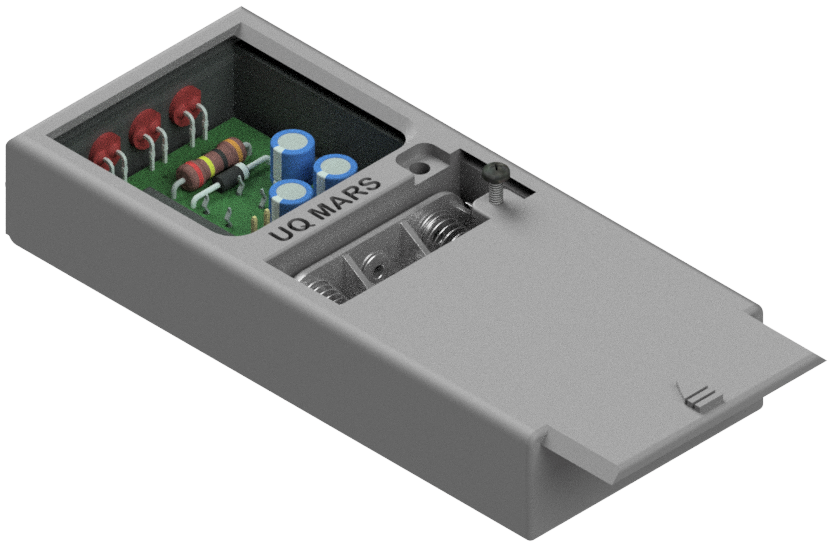
\includegraphics[width=0.99\linewidth]{Photos/Torch.png}
    \end{subfigure}
    \begin{subfigure}{0.32\linewidth}
        \includegraphics[width=0.99\linewidth]{Photos/CSIRO.jpg}
    \end{subfigure}
\end{figure}

\subsection*{Micromouse Competition}
The micromouse competition sees competitors design a small robot to solve a maze of which the path is randomised in the fastest time possible.
This compels competitors to utilise the best algorithms and design the fastest robot mice possible. We aim to host this competition in UQ Innovate and live-stream it through our YouTube channel.
There will be three main challenges:
\begin{itemize}
    \item Fastest time
    \item Cost Effectiveness 
    \item Going over correct checkpoints and avoiding others
\end{itemize}
While the \textit{cheapest design} challenge can be done in tandem, the other two challenges will be separate races. We believe these three challenges will produce unique designs and all some flavour to a competition first held in the 1970`s.

To ensure that our competition is up to international standards, we are in contact with IEEE, Techfest, UK Micromouse and Robotics Society, and Lunghwa University of Science and Technology. 
    
\newpage

\subsection*{Workshops}

Workshops have been at the heart of our society's events. They help our members gain skills they otherwise wouldn't for both professional and personal use.
Where possible, we will be recording our workshops and uploading them to our YouTube account for members' future reference.

\begin{itemize}
    \item PCB Design   
    \item Mechanical CAD Design
    \item Microcontroller Utilisation
    \item Sensor Synthesis
    \item Computer Vision
    \item Path Planning Algorithms
    \item Control System Simulation
\end{itemize}

\begin{figure}[H]
    \centering
    \includegraphics[width=0.42\linewidth]{prospectus/2024/Photos/CAD-3.jpg}
    \includegraphics[width=0.42\linewidth]{prospectus/2024/Photos/PCB-04.jpg}
    \includegraphics[width=0.42\linewidth]{prospectus/2024/Photos/CAD-8.jpg}
    \includegraphics[width=0.42\linewidth]{prospectus/2023/Photos/Hackathon.jpg}
\end{figure}


\newpage

\subsection*{Microcontroller Hackathon}
Each year, we host a Hackathon in conjunction with Robogals and QUT Robotics.
The event starts with an introduction night, which allowed students the opportunity to network and form teams.
The event pushes for students to connect and form lasting relationships with students from other universities, and develop new skills around embedded technology through project-based learning with Arduinos (such as programming control systems in C++).
Each society will bring one sponsor to judge each team`s project. Each year there is a theme for students to use as a guide.
One outcome of this annual event, is to provide Robogals new material to teach at their workshops aimed at inspiring young women to join STEM.

% ----- REPLACE IMAGE -----------------%
\begin{figure}[H]
    \centering
    \includegraphics[width=0.9\linewidth]{Photos/Arduino1.jpg}
\end{figure}


\subsection*{Regular Talks and Seminars} 
As a means to introduce members to some of the more obscure and interesting applications of mechatronics and robotics, we plan to make our hosted talks and seminars a regular feature.
These events are presented by researchers, students and industry professionals in fields that they have experience / interest in.

\subsection*{Community Outreach}
We hope to inspire the engineers of tomorrow through outreach workshops intended to introduce current high school students to the fields of mechatronics and robotics.
We will involve members within the running of these workshops to help them with the development of their own interpersonal skills.

\subsection*{Inter-Society and Inter-University Events}
We understand that tertiary study is more than your classes, it's also the connections and friendships you make while undertaking study.
Next year, we are committed to building strong relationships with other student societies both at the University of Queensland and elsewhere.
As part of this commitment we will be running and hosting a '\textit{Show and Tell}' night for members of UQ STEM Societies to show of their personal projects.

\subsection*{Mechatronics Study Guide}
We are currently developing a comprehensive course guide to aid students in the selection of their courses.
The guide will present suggested program structures, enrolment plans, course profiles, and offer the chance to inform students of the specific pathways available within Mechatronics and adjacent specialisations such as Electrical/Computer Engineering.
We will aim to give specialised advice from our executive team and various UQ MARS Alumni regarding study advice, course selection and general career advice.

\subsection*{Projects \& Competitions}
The most valuable skill that any engineer can gain is the ability to design elegant solutions to problems in the real world, that is why in 2024 with the help of our partners there is a plethora of competitions internationally and globally that UQ MARS has expressions of interest to compete in for many robotics based challenges. Alongside this is a list of in house projects that our executive team has worked tirelessly to manage and with support in 2024 these can be achieved in both the short term and long term and adds a level of engagement to our society that we believe will greatly benefit not only our members but our partners.

\begin{figure}[H]
    \centering
    \includegraphics[width=0.65\linewidth]{Photos/HardAF.jpg}
\end{figure}

\newpage

\section*{Partnering with UQ MARS}
\large
We offer a number of sponsorship packages which are laid out below. The prices provided are annual figures, quoted in AUD.
\normalsize

\subsection*{
    
\includegraphics[width=1em]{../assets/Sponsor Icons/Bronze.png}
    \textcolor{sponsor_bronze}{Bronze Tier (\$250)}
}
Bronze Tier sponsorship will have you:
\begin{itemize}
    \item Listed on the club website
    \item Advertisement of opportunities on all of our social media platforms to undergraduates and postgraduates alike
    \item Up to two representatives at any of our networking events
\end{itemize}

\subsection*{
    
\includegraphics[width=1em]{../assets/Sponsor Icons/Silver.png}
    \textcolor{sponsor_silver}{Silver Tier (\$1000)}
}
Silver Tier sponsorship will include the perks of Bronze Tier, including the opportunity to collaborate with UQ MARS in the following ways:
\begin{itemize}
    \item Present one of our regular talks / seminars
    \item Send representation to one of our industry events (such as panels or networking nights)
    \item Or
    \item Use of their product as a core component in a workshop (which should also be recorded and published in future)
\end{itemize}

\subsection*{
    
\includegraphics[width=1em]{../assets/Sponsor Icons/Gold}
    \textcolor{sponsor_gold}{Gold Tier (\$4000)}
}
Gold Tier sponsorship entitles you to all of the available perks of Silver Tier, in addition to the following:
\begin{itemize}
    \item Have a representative sit on the judging panel for one of our key events being:
    
    \begin{itemize}
        \item Microcontroller Hackathon
        \item Micromouse
    \end{itemize}
    
    \item Host a dedicated event with us to promote your organisation and present opportunities to future Engineers.  
    
    \item Your company Logo presented on our competition uniforms, these competitions include but are not limited to: 
    \begin{itemize}
        \item Droid Race Competition
        \item Roborave Australia 
    \end{itemize}
\end{itemize}

\subsection*{
    
\includegraphics[width=1em]{../assets/Sponsor Icons/Turbo.png}
    \textcolor{turbo_purple}{Turbo Tier (\$10,000)}
}
Turbo Tier sponsorship is our most comprehensive package, entitling you to all of the perks of Gold Tier, with the added benefit of being the sole partner in one of the following events hosted by our Society:
\begin{itemize}
    \item Microcontroller Hackathon 
    \item UQ MARS Micromouse 
    \item UQ MARS Outreach Program 
\end{itemize}

\subsection{\textit{*Disclaimer}}
Should your organisation choose to become a partner with UQ MARS in 2024 it follows that there are limited positions available for perks such as judges and guest events and thus we will operate on a first come first serve basis for all partners. If in the event that a perk has been allotted all vacant positions this will be communicated before any official proceedings are made. Alongside this if you wish to have your organisations logo presented on our competition uniforms we ask that this be known prior to the end of February 2024 as this is when the yearly order is placed.

\newpage

\section*{Contact Us}
\begin{figure}[H]
    \centering
    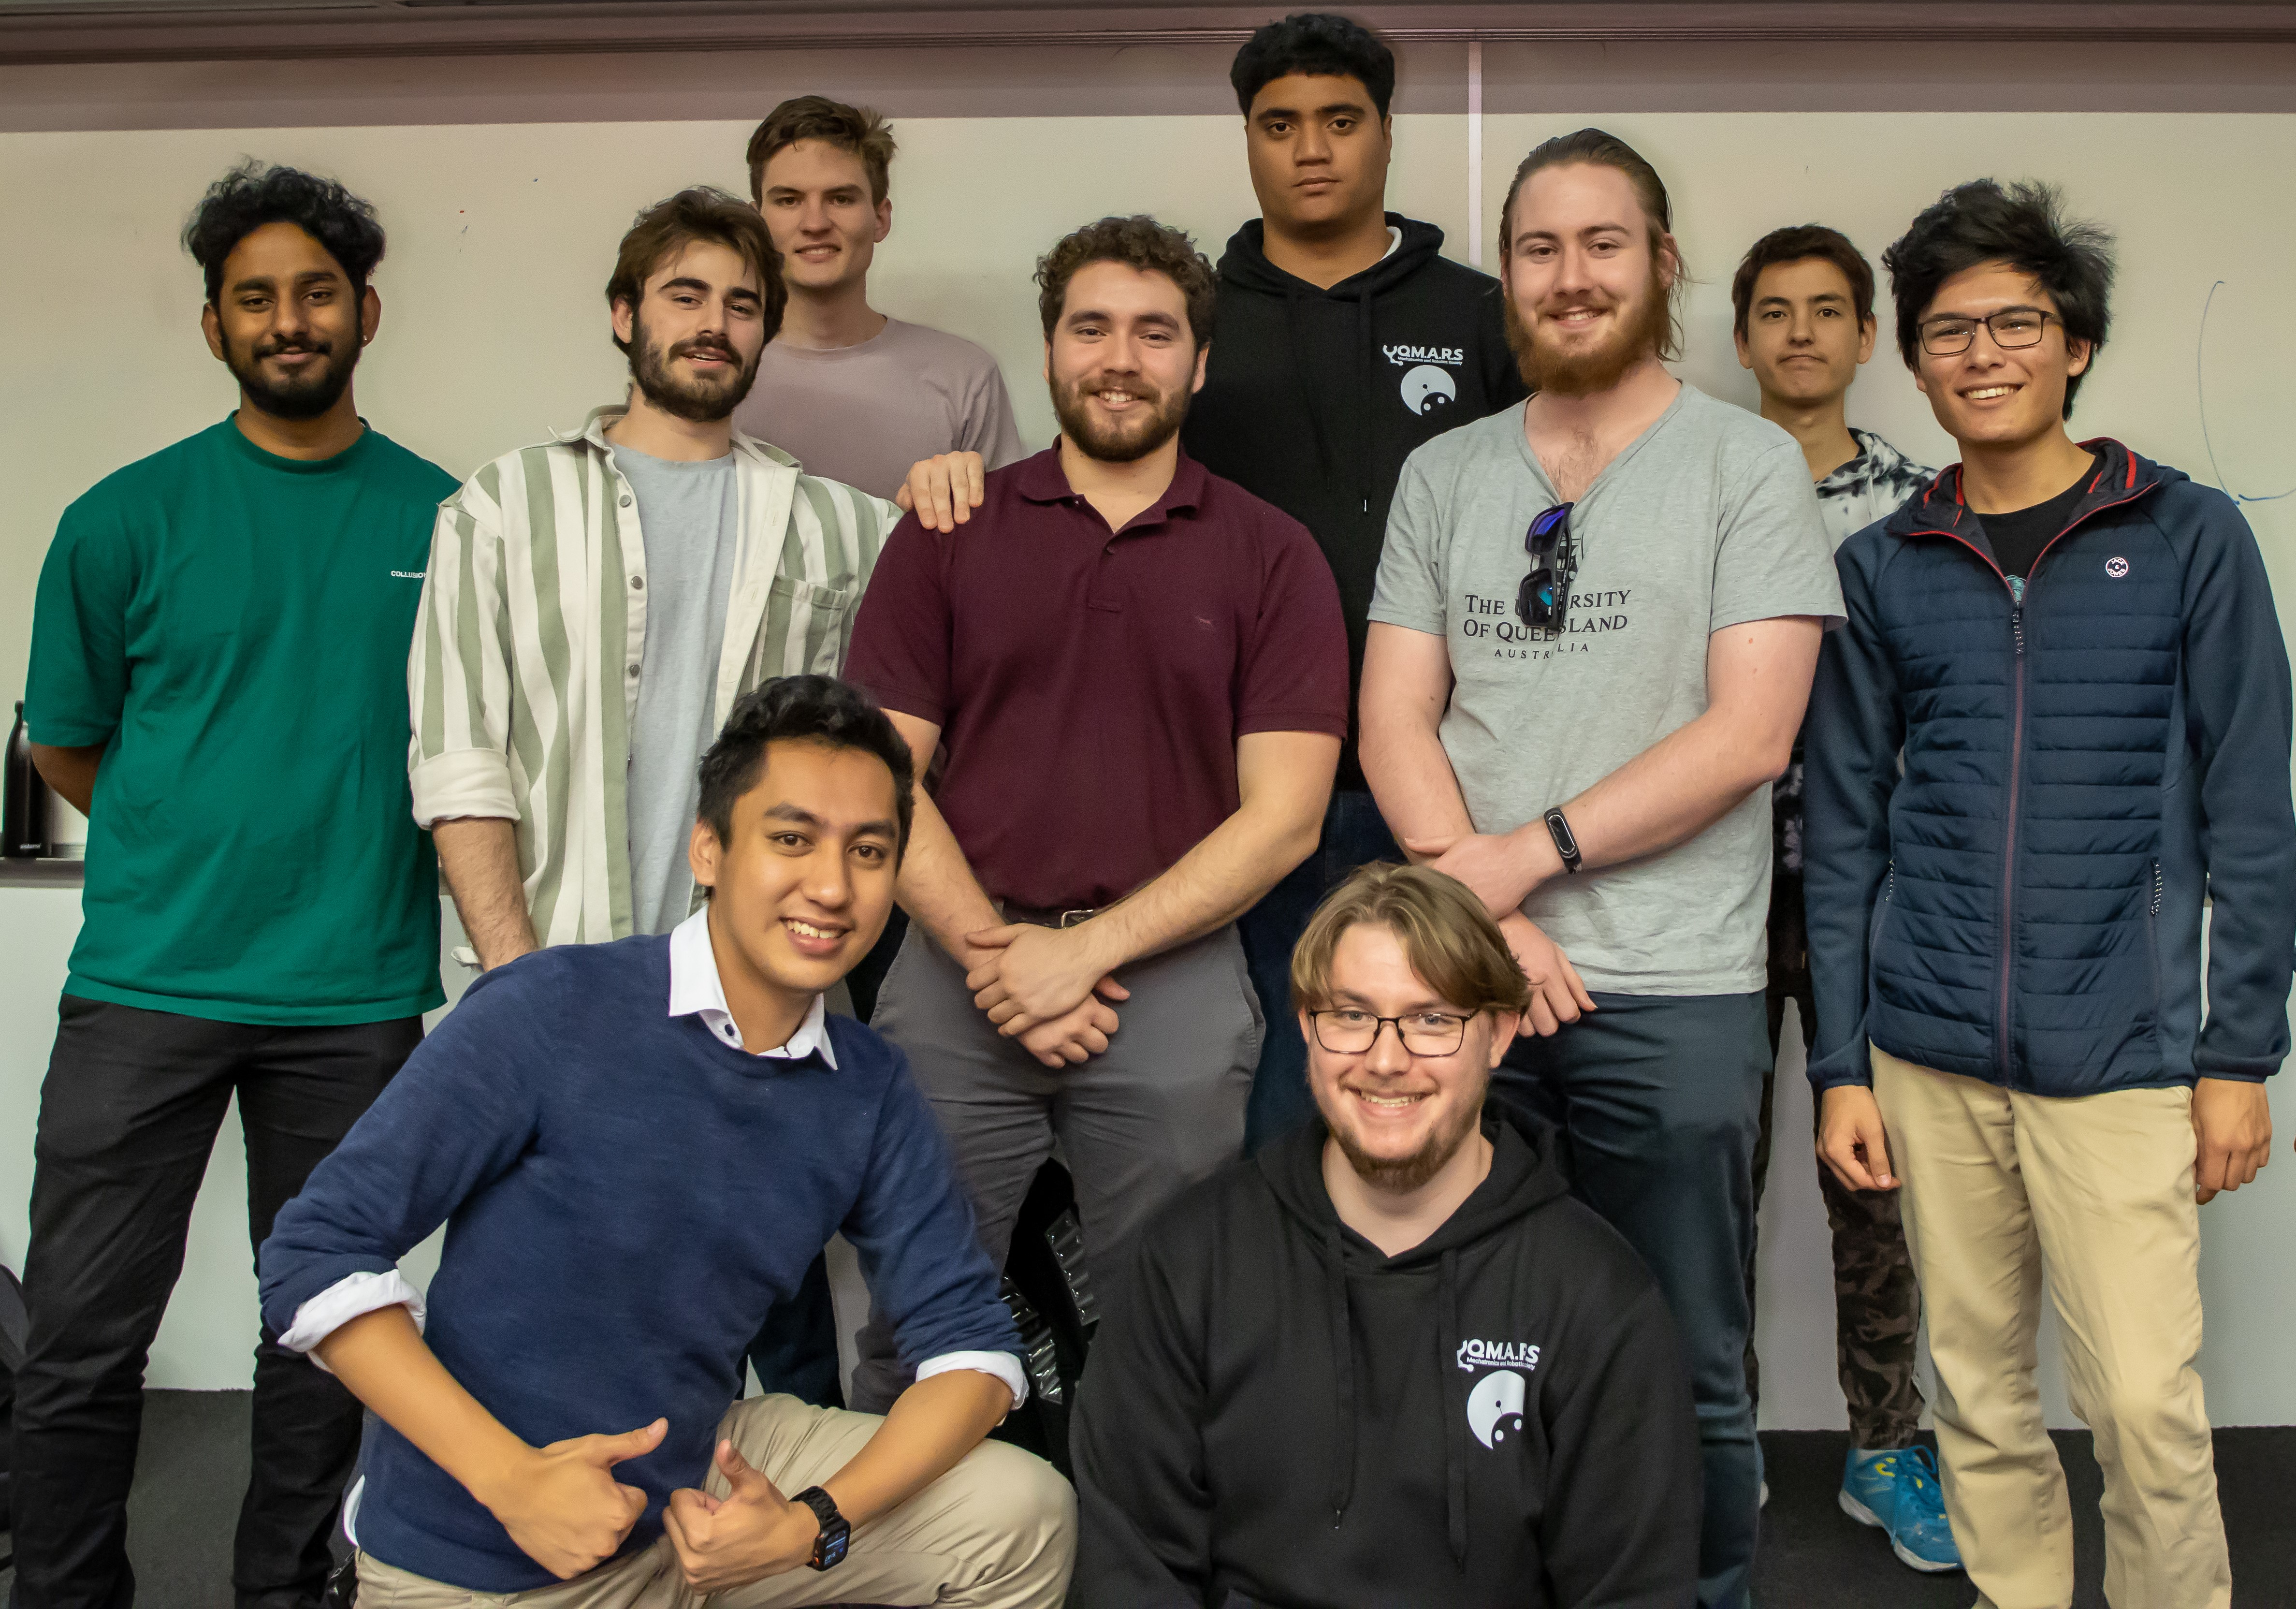
\includegraphics[width=0.9\linewidth]{Photos/Exec.jpg}
\end{figure}

\large
\onehalfspacing
You can contact us through any of the following platforms: \\
\faLink{} \href{https://www.uqmars.com}{uqmars.com} \\
\faEnvelope{} \href{mailto:partnerships@uqmars.com}{partnerships@uqmars.com} \\
\faFacebookSquare{} \href{https://facebook.com/UQMARS}{UQ MARS} \\
\faLinkedinSquare{} \href{https://linkedin.com/company/uq-mars}{UQ Mechatronics and Robotics Society (UQ MARS)} \\
\faGithubSquare{} \href{https://github.com/uqmars}{UQ Mechatronics And Robotics Society} \\
\faYoutubePlay{} \href{https://www.youtube.com/channel/UCH3GjoKLL3R_1ayjkn9C78A}{UQ MARS} \\
\faInstagram{} \href{https://www.instagram.com/uq.mars/}{uq.mars} \\
We look forward to hearing from you!

\end{document}
